\chapter{Data}
\label{c:data}
\index{data|hyperbf}

A \tao \vn{``datum''} is a parameter associated with a lattice that is used in lattice correction or
design (\sref{c:opti}). Example data includes the vertical orbit at a particular position or the
horizontal emittance of a storage ring. This chapter explains how data is organized in \tao while
Section~\sref{s:init.data} explains how, in an initialization file, to define the structures that
hold the data.  When running \tao, the \vn{show data} (\sref{s:show}) command can be used to view
information about the data.

%------------------------------------------------------------------------
\section{Data Organization}
\label{s:data.org}

\begin{figure}
  \centering
  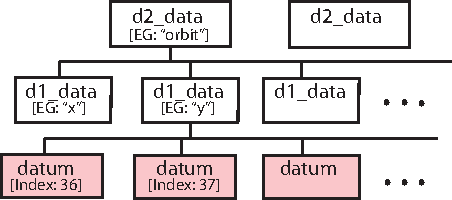
\includegraphics[width=4in]{data-tree.pdf}
  \caption[Data tree structure]
{A \vn{d2_data} structure holds a set of \vn{d1_data} structures. 
A \vn{d1_data} structure holds an array of datums.}
  \label{f:data.tree}
\end{figure}

\index{d2_data}\index{d1_data}
The horizontal orbit at a particular BPM is an example of an individual \vn{datum}. For ease of
manipulation, arrays of datums are grouped into what is called a \vn{d1_data}
structure. Furthermore, sets of \vn{d1_data} structures are grouped into what is called a
\vn{d2_data} structure.  This is illustrated in Figure~\ref{f:data.tree}.  For example, a
\vn{d2_data} structure for orbit data could contain two \vn{d1_data} structures --- one \vn{d1_data}
structure for the horizontal orbit data and another \vn{d1_data} structure for the vertical orbit
data. Each datum of, say, the horizontal orbit \vn{d1_data} structure would then correspond to the
horizontal orbit at some point in the machine. 

When issuing \tao commands, all the data associated with a \vn{d2_data} structure is specified using
the \vn{d2_data} structure's \vn{name}.  The data associated with a \vn{d1_data} structure is
specified using the format
\begin{example}
  d2_name.d1_name
\end{example}
For example, if a \vn{d2_data} structure has the name ``\vn{orbit}'', and one of its \vn{d1_data}
structures has the name ``\vn{x}'', then \tao commands that refer to the data in this \vn{d1_data}
structure use the name ``\vn{orbit.x}''. Sometimes there is only one \vn{d1_data} structure for a
given \vn{d2_data} structure. In this case the data can be referred to simply by using the
\vn{d2_data} structure's name. The individual datums can be referred to using the notation
\begin{example}
  <d2_name>.<d1_name>[<list_of_datum_indexes>]
\end{example}
For example, \vn{orbit.x[10]} refers to the horizontal orbit datum with index 10. Notice that the
beginning (lowest) datum index is user selectable and is therefore not necessarily 1.

Period characters are not allowed in both the \vn{d2_data} and \vn{d1_data} names.

It is important to note that the name given to \vn{d2_data} and \vn{d1_data} structures is arbitrary
and does not have to correspond to the type of data contained in the structures. In fact, a
\vn{d1_data} array can contain heterogeneous data types.  Thus, for example, it is perfectly
permissible (but definitely not recommended) to set up the data structures so that, say,
\vn{orbit.x[10]} is the $a$-mode emittance at a certain element and \vn{orbit.x[11]} is the $b$-mode
beta function at the same element.

Ranges of data can be referred to using using a comma \vn{,} to separate the indexes combined with
the notation \vn{n1:n2} to specify all the datums between \vn{n1} and \vn{n2} inclusive. For example
\begin{example}
  orbit.x[3:6,23]
\end{example}
refers to datums 3, 4, 5, 6, and 23. 

If multiple universes are present, each universe will have its own set of \vn{d2_data}
structures. The name of a particular \vn{d2_data} structure may be the same as a \vn{d2_data}
structure in a separate universe. So, for example, an \vn{orbit} \vn{d2_data} structure may
be present in multiple universes.

As explained in \sref{s:universe}, the prefix \vn{"@"} may
be used to specify which universe the data applies to. The general notation is
\begin{example}
  [<universe_range>]@<d2_name>.<d1_name>[<datum_index>]
\end{example}
Examples:
\begin{example}
  [2:4,7]@orbit.x ! The \vn{orbit.x} data in universes 2, 3, 4 and 7.
  [2]@orbit.x     ! The \vn{orbit.x} data in universe 2. 
  2@orbit.x       ! Same as "2@orbit.x".
  orbit.x         ! The \vn{orbit.x} data in the current default universe.
  -1@orbit.x      ! Same as "orbit.x".
\end{example}

As explained in Section~\sref{s:data.anatomy}, each individual datum has a number of components. The
syntax to refer to a component is:
\begin{example}
  d2_name.d1_name[datum_index]|component
\end{example}
For example:
\begin{example}
  orbit.x[3:10]|meas     ! The measured data values
\end{example}

In referring to datums, a ``\vn{*}'' can be used as a wild card to 
denote ``all''. Thus:
\begin{example}
  *@orbit.x       ! The \vn{orbit.x} data in all universes.
  *               ! All the data in the current default universe.
  *.*             ! Same as "*"
  *@*             ! All the data in all the universes. 
  *@*.*           ! Same as "*@*"
  orbit.x[*]|meas ! All measured values of orbit.x
  orbit.x[]|meas  ! No values. That is, the empty set.
  orbit.x|meas    ! Same as orbit.x[*]|meas.
\end{example}
The last example shows that when referring to an entire block of data
encompassed by a \vn{d1_data} structure, the \vn{[*]} can be omitted.

%------------------------------------------------------------------------
\section{Anatomy of a Datum}
\label{s:data.anatomy}

Each datum has a number of components associated with it:
\begin{example}
  data_type        ! Character: Type of data: "orbit.x", etc.
  ele_name         ! Character: Name of lattice element where datum is evaluated at.
  ele_start_name   ! Character: Name of starting lattice element in a range.
  ele_ref_name     ! Character: Name of reference lattice element.
  merit_type       ! Character: Type of constraint: "target", "max", etc.
  data_source      ! Character: How the datum is calculated. "lat", "beam", etc.
  ix_ele\Ss          ! Integer: Index of "ele" in the lattice element list.
  ix_branch\Ss        ! Integer: Lattice branch index.
  ix_ele_start\Ss     ! Integer: Index of "ele_start" in the lattice element list.
  ix_ele_ref\Ss       ! Integer: Index of "ele_ref" in the lattice element list.
  ix_ele_merit\Ss     ! Integer: Lattice index where merit is evaluated.
  ix_d1\Ss            ! Integer: Index number in d1_data structure
  ix_data\Ss          ! Integer: Index in the global data array
  ix_dModel\Ss        ! Integer: Row number in the dModel_dVar derivative matrix.
  ix_bunch         ! Integer: Bunch number to get the data from.
  eval_point       ! Character/integer: Evaluation point relative to the lattice element.
  meas             ! Real: Measured datum value. Set by the User.
  ref              ! Real: Measured datum value from the reference data set. Set by the User.
  model\Ss            ! Real: Datum value as calculated from the model.
  design\Ss           ! Real: What the datum value is in the design lattice.
  old\Ss              ! Real: Used by \tao to save the model at some previous time.
  base\Ss             ! Real: The value as calculated from the base model.
  fit\Dd              ! Real: This value is not used by \tao.
  invalid          ! Real: The value used for delta_merit if good_model = False.
  error_rms        ! Real: Measurement error. Used for plotting.
  delta_merit\Ss      ! Real: Diff used to calculate the merit function term.
  weight           ! Real: Weight for the merit function term
  merit\Ss            ! Real: Merit function term value: weight * delta^2
  s\Ss                ! Real: longitudinal position of ele.
  s_offset         ! Real: Offset of the evaluation point.
  spin_axis        ! Structure: Used for Spin G-matrix calculations.
  exists\Ss           ! Logical: Does the datum exist?
  good_model\Ss       ! Logical: Does the model  component contain a valid value?
  good_design\Ss      ! Logical: Does the design component contain a valid value?
  good_base\Ss        ! Logical: Does the base   component contain a valid value?
  good_meas        ! Logical: Does the meas   component contain a valid value?
  good_ref         ! Logical: Does the ref    component contain a valid value?
  good_user        ! Logical: Does the user want this datum used in optimization?
  good_opt\Dd         ! Logical: Similar to good_user. Can be used in Tao extensions.
  good_plot\Dd        ! Logical: Is datum within the horizontal extent of the plot?
  useit_plot\Ss       ! Logical: Is this datum to be used in plotting?
  useit_opt\Ss        ! Logical: Is this datum to be used for optimization?
\end{example}
\Ss Set by \tao. \Dd Used by \tao extensions. Not user settable.

When running \tao, the \vn{show data} (\sref{s:show}) command can be used to view the components of a datum. 
The \vn{set} command (\sref{s:set}) can be used to set some of these components.
Note: Some of these components are set by the user and some of these components will be calculated by
\tao. A description of what components can be set is given in \Sref{s:init.data}.

\begin{description}
  \item[base] \Newline
The value of the datum as calculated from the base lattice (\sref{s:datum.values}).
%
  \item[data_source] \Newline
The \vn{data_source} component specifies where the data is coming from
(\sref{s:data.source}).
%
  \item[data_type] \Newline
The type of data (\sref{s:data.types}). For example, \vn{beta.a}. At startup, if the
\vn{data_type} is not specified, it is set to \vn{<d2_name>.<d1_name>} where
\vn{<d2_name>} is the name of the associated \vn{d2} data structure and \vn{<d1_name>} is 
the name of the associated \vn{d1} data structure (\sref{s:init.data}).
%
  \item[delta_merit] \Newline
Difference used to calculate the contribution of the datum to the merit function (\sref{s:lat.correction}).
%
  \item[design] \Newline
The value of the datum as calculated from the design lattice (\sref{s:datum.values}).
%
  \item[ele_name] \Newline
Name of the associated lattice element where the datum is evaluated at (\sref{s:data.lat.ele}) or,
if \vn{ele_start_name} is set, the last element in the evaluation range. Not used for datums that
are \vn{global}, like the emittance. Also see \vn{eval_point} and \vn{s_offset} components.
%
  \item[ele_start_name] \Newline
Starting element of a range of lattice elements (\sref{s:data.lat.ele}).
%
  \item[ele_ref_name] \Newline
Reference lattice element (\sref{s:data.lat.ele}). Not to be confused with the \vn{ref} component
which is a user settable value.
%
  \item[error_rms] \Newline
The error associated with the measured or reference data values. Used for drawing error bars. See the 
documentation on \vn{curve(N)%draw_error_bars} in \Sref{s:template}.
for more details.
%
  \item[eval_point] \Newline
Set to "\vn{beginning}", "\vn{center}", or "\vn{end}". Used with \vn{s_offset} to determine where
the datum is evaluated at (\sref{s:dat.eval}). The evaluation point will be ignored if using an
evaluation range (\vn{ele_start_name} is set) is used.
%
  \item[exists] \Newline
Set by \tao to True if the datum exists (\sref{s:datum.opt}). 
%
  \item[fit] \Newline
Not used by \tao. Can be used with custom code.
%
  \item[good_base] \Newline
Set by \tao. Is the \vn{base} value valid?
%
  \item[good_design] \Newline
Set by \tao. Is the value as calculated from the \vn{design} lattice valid? For example, if the
datum is the particle orbit at some BPM in a ring and if it is not possible to compute the orbit at
the BPM due to the lattice being unstable then \vn{good_design} will be False.
%
  \item[good_meas] \Newline
Set by \tao. Is the \vn{meas} value valid?
%
  \item[good_model] \Newline
Set by the user. Is the value as calculated from the \vn{model} lattice valid? For example, if the
datum is the particle orbit at some BPM in a lattice with open geometry and if it is not possible to
compute the orbit at the BPM due to the particle being lost upstream of the element then
\vn{good_model} will be False.
%
  \item[good_opt] \Newline
Set by the user. This component is similar \vn{good_user} except that it is unaffected by the
\vn{veto}, \vn{restore} and \vn{use} commands.
%
  \item[good_plot] \Newline
Set by Tao. Is datum within the horizontal extent of the plot? 
%
  \item[good_ref] \Newline
Set by the user. Is the \vn{ref} value valid?
%
  \item[good_user] \Newline
Set by the user. Is the datum valid for optimization or plotting? Use the commands \vn{veto}, \vn{restore},
\vn{use} and \vn{set data} to set while running \tao.
%
  \item[invalid] \Newline
The value used in the computation of \vn{delta_merit} one of the following three conditions is
True: 1) if \vn{good_model} = False, or 2) if \vn{good_base} is False when the global \vn{opt_with_base}
is True, or 3) if \vn{good_design} is False when the global \vn{opt_with_ref} is True.
%
  \item[ix_branch] \Newline
The index of the lattice branch that contains \vn{ele}, \vn{ref_ele}, and \vn{start_ele}.
%
  \item[ix_ele] \Newline
Index of the lattice element where the datum is evaluated at. 
%
  \item[ix_ele_start] \Newline
Index of the start element.
%
  \item[ix_ele_ref] \Newline
Index of the reference element.
%
  \item[ix_ele_merit] \Newline
Set by \tao. When the \vn{merit_type} is set to \vn{max} or \vn{min} and there is a range
of elements that over which the there is an evaluation, ix_ele_merit is set to the element
where the value is the \vn{max} or \vn{min}.
%
  \item[ix_d1] \Newline
Index of the associated \vn{d1_data} array.
%
  \item[ix_data] \Newline
For convenience, all the datums of a given universe are put into one large array. \vn{ix_data} is the index
of the datum in this array. This is useful for debugging purposes.
%
  \item[ix_dModel] \Newline
For optimization, \tao creates a derivative matrix dMerit_i/dVar_j. \vn{ix_dmodel} is set
to the i\Th column of this matrix. This is useful for debugging purposes
%
  \item[ix_bunch] \Newline
For datums that have \vn{data_source} set to \vn{beam}, \vn{ix_bunch} selects which bunch
of the beam the datum is evaluated at.
%
  \item[meas] \Newline
The value of the datum as obtained from some measurement (\sref{s:datum.values}).
%
  \item[merit] \Newline
The contribution to the merit function due to this datum (\sref{s:lat.correction}).
%
  \item[merit_type] \Newline
The type of merit (\sref{s:del.d}). Possible values are:
\begin{example}
  "target"
  "min",     "max"
  "abs_min", "abs_max"
  "max-min"                     ! Only used when datum specifies a range of elements.
  "average", "integral", "rms"  ! Only used when datum specifies a range of elements.
\end{example}
%
  \item[model] \Newline
The value of the datum as calculated from the \vn{model} lattice (\sref{s:datum.values}).
%
  \item[old] \Newline
A datum value that was saved at some point in \tao's calculations. This value
can be ignored (\sref{s:datum.values}).
%
  \item[ref] \Newline
The reference datum value as obtained from some reference measurement (\sref{s:datum.values}).
Set by the User. Not to be confused with the reference element.
%
  \item[s] \Newline
Longitudinal $s$-position of the lattice element.
%
  \item[s_offset] \Newline
Offset of the evaluation point when there is an associated lattice element (\sref{s:dat.eval}).
The offset will be ignored if using an evaluation range (\vn{ele_start_name} is set) is used.
%
  \item[spin_axis]
The \vn{spin_axis} component is a structure used for Spin G-matrix calculations
(\vn{spin_g_matrix.$ij$} data type). \vn{Spin_axis} gives the $(l, n_0, m)$ coordinate axes at the
reference element. See \sref{s:init.data} for documentation on how to set this structure.
%
  \item[useit_opt] \Newline
Datum is used for optimization. \vn{useit_opt} is set by \tao using the other
\vn{logicals} components using the prescription:
\begin{example}
  useit_opt = exists \& useit_opt \& good_user \& good_meas \& 
              good_ref (if reference data is used in optimization)
Notice that if, for example, \vn{good_model} is False then the datum will still be used for optimization but
in this case the \vn{invalid} value set by the user will be used in the computation for \vn{delta_merit} in
place of a value computed from lattice.
\end{example}
%
%
  \item[useit_plot] \Newline
Set \vn{True} if the datum is valid for plotting for a particular graph. This component gets
reevaluated for each \vn{graph} that potentially uses the datum so the value observed after plotting is
refreshed is simply the value as calculated for the last \vn{graph} considered. The value for \vn{useit_plot}
is evaluated using other logical components using the prescription:
\begin{example}
  useit_plot = exists \& good_plot \& 
                  (good_user | graph:draw_only_good_user_data_or_vars) \&
                  good_meas (if measured data is being plotted) \& 
                  good_ref (if reference data is being plotted) \&
                  good_model (if model data is being plotted)
\end{example}
%
  \item[weight] \Newline
Weight used in evaluating the contribution of the datum to the merit function (\sref{s:lat.correction}).
\end{description}

%------------------------------------------------------------------------
\section{Datum values}
\label{s:datum.values}

\index{data!measured}\index{data!reference}\index{data!model}
\index{data!base}\index{data!design}
A given datum has six values associated it:
\vspace{-2ex}
\begin{description}
  \vspace{-1ex}
  \item[meas] \Newline 
When fitting data, the \vn{meas} value is the value of the datum as obtained from some
measurement. When designing lattices, the \vn{meas} value is the desired value of the datum. For
example, when designing a lattice for a colliding ring machine, a datum may be constructed for 
the beta function at the interaction point with the \vn{meas} value set to the desired value. See
Chapter~\ref{c:opti} for more details.
  \vspace{-1ex}
  \item[base] \Newline
The datum value as calculated from the \vn{base} lattice (\sref{s:lattice}).
  \vspace{-0.5ex}
  \item[design] \Newline
The value of the datum as calculated from the \vn{design} lattice (\sref{s:lattice}).
  \vspace{-0.5ex}
  \item[fit] \Newline
The \vn{fit} value is not used by \tao directly and is available for use by custom code.
  \vspace{-0.5ex}
  \item[model] \Newline
The value of the datum as calculated from the \vn{model} lattice (\sref{s:lattice}).
  \vspace{-0.5ex}
  \item[old] \Newline
A datum value that was saved at some point in \tao's calculations. This value
can be ignored.
  \vspace{-0.5ex}
  \item[ref] \Newline
When fitting data, \vn{ref} is the datum value as obtained from some reference measurement. For
example, a measurement before some variable is varied could be designated as the \vn{reference}, and
the datum taken after the variation could be designated the \vn{measured} datum. When designing
lattices, the \vn{ref} value is the value of the datum associated with the \vn{design} or \vn{base}
lattice (determined by the setting of the global \vn{opt_with_base} parameter
(\sref{s:del.d}). Note: The \vn{meas} value of a datum is always associated with the
\vn{model} lattice.
\end{description}

%------------------------------------------------------------------------
\section{Evaluation Point of a Datum}.
\label{s:dat.eval}

When the datum is to be evaluated at a specific point in the lattice, that is, when there
is an associated lattice element, the default position for evaluating the datum is at the
downstream end of the element. This evaluation point can be shifted using the
\vn{eval_point} and/or \vn{s_offset} components. 

The \vn{eval_point} component can be set to one of:
\begin{example}
  beginning   ! entrance end of lattice element.
  center      ! Center of lattice element
  end         ! Exit end of lattice element. Default.
\end{example}
The evaluation point is shifted by \vn{s_offset} from the \vn{eval_point}.

If there is a reference point, the setting of \vn{eval_point} is used to determine where
the reference point. The setting of \vn{s_offset} is ignored for the reference point.

Due to internal logic considerations, Not all \vn{data_type}s are compatible with a finite
\vn{s_offset} or a setting of \vn{eval_point} to \vn{center}. The table of \vn{data_type}s
(\sref{t:data.types}) shows which \vn{data_type}s are compatible and which are not.

Another restriction is that specifying a range of elements for evaluation (that is,
specifying \vn{ele_start_name} \sref{s:init.data}) is not compatible with a finite
\vn{s_offset} or a setting of \vn{eval_point} to \vn{center}.

%------------------------------------------------------------------------
\section{Datums in Optimization}
\label{s:datum.opt}

When using optimization for lattice correction or lattice design (\sref{c:opti}), Individual datums
can be excluded from the process using the \vn{veto} (\sref{s:veto}), \vn{restore}
(\sref{s:restore}), and \vn{use} (\sref{s:use}) commands. These set the \vn{good_user} component of
a datum. This, combined with the setting \vn{exists}, \vn{good_meas}, \vn{good_ref}, and
\vn{good_opt} determine the setting of \vn{useit_opt} which is the component that determines if the
datum is used in the computation of the merit function. The settings of everything but
\vn{good_user} is determined by \tao. The value of \vn{good_user} for a datum can be set in an
initialization file (\sref{s:init.data}) or on the command line using the \vn{use}, (\sref{s:use}) \vn{veto} (\sref{s:veto}), or
\vn{restore} (\sref{s:restore}) commands.

The \vn{exists} component is set by \tao to True if the datum exists and False otherwise. A datum
may not exist if the type of datum requires the designation of an associated element but the
\vn{ele_name} component is blank. For example, a \vn{d1_data} array set up to hold orbit data may
use a numbering scheme that fits the lattice so that , say, datum number 34 in the array does not
correspond to an existing BPM.

The \vn{good_model} component is set according to whether a datum value can be computed from the
\vn{model} lattice. For example, If a circular lattice is unstable, the beta function and the closed
orbit cannot be computed. Similarly, the \vn{good_design} and \vn{good_base} components mark whether
the \vn{design} and \vn{base} values respectively are valid.

The \vn{delta_merit} component of a datum is set to the \vn{delta} value used in computing the
contribution to the merit function (\sref{s:del.d}). If it is not possible to compute
the datum value, then the \vn{invalid} component is used for the computation of \vn{delta_merit}.
It is not possible to compute the datum value if one of the following three conditions is True: 1)
\vn{good_model} is False, 2) \vn{good_design} is False and the global \vn{opt_with_ref} is True, or
3) \vn{good_base} is False and the global \vn{opt_with_base} is True.

\vn{good_meas} is set True if the \vn{meas} component value is set in the data initialization file
(\sref{s:init.data}) or is set using the \vn{set} command (\sref{s:set}). Similarly, \vn{good_ref}
is set True if the \vn{ref} component has been set. \vn{good_ref} only affects the setting of
\vn{useit_opt} if the optimization is using reference data as set by the global variable
\vn{opt_with_ref} (\sref{s:globals}).

Finally \vn{good_opt} is meant for use in custom versions of \tao (\sref{c:custom.tao}) and is
always left True by the standard \tao code.

Example of using a \vn{show data} (\sref{s:show}) to check the logicals
in a datum:
\begin{example}
  Tao> show data 3@beta[1]

  Universe:   3
  %ele_name          = IP_L0
  %ele_ref_name      =
  %ele_start_name    =
  %data_type         = beta.a
      ... etc ...
  %exists            =  T
  %good_model        =  T
  %good_meas         =  F
  %good_ref          =  F
  %good_user         =  T
  %good_opt          =  T
  %good_plot         =  F
  %useit_plot        =  F
  %useit_opt         =  F
\end{example}
Here \vn{useit_opt} is False since \vn{good_meas} is False and \vn{good_meas} is False since the
\vn{meas} value of the datum (not shown) was not set in the \tao initialization file or set using
the \vn{set} command.

%------------------------------------------------------------------------
\section{Data_source}
\index{data!data_source}
\label{s:data.source}

The \vn{data_source} component specifies where the data is 
coming from. Possible values are:
\begin{example}
  "beam"        ! Data from from multiparticle beam distribution
  "data"        ! Data from from a \tao datum in a data array.
  "lat"         ! Data from from the lattice.
\end{example}
If \vn{data_source} is set to \vn{"beam"}, the data is calculated
using multiparticle tracking.  If \vn{data_source} is set to
\vn{"lat"}, the data is calculated using the ``lattice'' which here
means everything {\em but} multiparticle tracking In particular, the "\vn{lat}" \vn{data_source}
includes data derived from single particle tracking. For example, the
\vn{"beam"} based calculation of the emittance uses the bunch sigma
matrix obtained through multiparticle tracking. The \vn{"lat"} based
calculation of the emittance uses radiation integrals.

Some data types may be restricted as to which \vn{data_source} is
possible. For example, a datum with \vn{data_type} set to
\vn{n_particle_loss} must use \vn{"beam"} for the \vn{data_source}. 
Table~\ref{t:data.types} lists which \vn{data_source} values are valid
for what data types.

%------------------------------------------------------------------------
\section{Datum Evaluation and Associated Lattice Elements}
\index{data!associated lattice elements}
\label{s:data.lat.ele}

Datums can be divided up into two classes. In one class are the datums
that are \vn{``local''}, like the beam orbit, which need to be evaluated at
either a particular point are evaluated over some finite region of the
machine. Other datums, like the emittance, are \vn{``global''} and do not
have associated evaluation points.

As mentioned, \vn{local} datums may be evaluated at a specific point
or over some evaluation region, an evaluation region is used when, for
example, the maximum or minimum value over a region is wanted. To
specify an evaluation point, an \vn{evaluation element} must be
associated with a datum. The evaluation point will be at the exit end
of this element. To specify an evaluation region, a \vn{start element}
must also be associated with a datum along with the \vn{evaluation
element}. The evaluation region is from the exit end of the \vn{start
element} to the exit end of the \vn{evaluation element}.

In addition to the \vn{evaluation element} and the \vn{start element}, a \vn{local} datum may have
an associated \vn{reference element}.  A \vn{reference element} is used as a fiducial point and the
datum value is calculated relative to that point. For example, a datum value may be the position of
the \vn{evaluation element} relative to the position of the \vn{reference element}. The evaluation
point of a \vn{reference element} is the exit end of that element.

The components in a datum corresponding to the \vn{evaluation element}, the \vn{reference element},
and the \vn{start element}.  are shown in Table~\ref{t:datum.elements}.  These three elements may be
specified for a datum by either setting the name component or the index component of the
datum. Using the element index over the element name is necessary when more than one element in the
lattice has the same name.

\begin{table}[htb]
\centering
\begin{tabular}{lll}
  \toprule
  &\multicolumn{2}{c}{\it Data Component} \\ \cmidrule{2-3}
  {\it Element} & {\it name} & {\it index} \\ \midrule
  Reference Element  & \vn{ele_ref_name}   & \vn{ix_ele_ref}   \\
  Start Element      & \vn{ele_start_name} & \vn{ix_ele_start} \\
  Evaluation Element & \vn{ele_name}       & \vn{ix_ele}       \\ \bottomrule
\end{tabular}
\caption[The three lattice elements associated with a datum.]  {The three lattice elements
associated with a datum may be specified in the datum by setting the appropriate name component or
by setting the appropriate index component.}  \label{t:datum.elements}
\end{table}

If a datum has an associated \vn{evaluation} element, but no associated \vn{start} or \vn{reference}
elements, the \vn{model} value of that datum is the value of the \vn{data_type} at the
\vn{evaluation} element. For example, if a datum has:
\begin{example}
  data_type      = "orbit.x"
  ele_name       = "q12"
\end{example}
here the \vn{model} value of this datum will be the horizontal orbit at the element with name
\vn{q12}.

If a datum has an associated \vn{start} element, specified by either setting the \vn{ele_start_name}
or \vn{ix_ele_start} datum components, the datum is evaluated over a region from the exit end of the
\vn{start} element to the exit end of \vn{evaluation} element. For example, if a datum has:
\begin{example}
  data_type      = "beta.a"
  ele_name       = "q12"
  ele_start_name = "q45"
  merit_type     = "max"
\end{example}
then the \vn{model} value of this datum will be the maximum value of the a-mode beta function in the
\vn{model} lattice in the region from the exit end of the element with name \vn{q12} to the exit end
of the element with name \vn{q45}. The \vn{base} and \vn{design} values are computed similarly using
the \vn{base} and \vn{design} lattices. 

If the lattice branch associated with the datum has a closed geometry, and if the lattice element
associated with \vn{ele_start_name} is after the element specified by \vn{ele_name}, the evaluation
region will be the region from \vn{ele_start_name} to the end of the branch along with the region
from the beginning of the branch to the element specified by \vn{ele_name}. That is, the evaluation
region ``wraps'' around the end of the lattice.  

It does not make sense to specify an evaluation range when the datum's \vn{merit_type} is set to
\vn{"target"}. In this case, the \vn{model}, \vn{base}, and \vn{design} values are the value of the
datum at the evaluation element. Also notice that for datums that do not have an evaluation element,
for example, if \vn{data_type} is set to \vn{"emit.a"}, specifying an evaluation range does not make
sense.

Typically, in evaluating a datum over some region to find the maximum or minimum, \tao will only
evaluate the datum at the ends of the elements with the assumption that this is good enough. If this
is not good enough, marker elements can be inserted into the lattice at locations that matter. For
example, the maximum or minimum of the beta function typically occurs near the middle of a
quadrupole so inserting marker elements in the middle of quadrupoles will improve the accuracy of
finding the extremum beta.

If a datum has an associated \vn{reference} element, specified by either setting the
\vn{ele_ref_name} or \vn{ix_ele_ref} datum components, the \vn{model} value of the datum is the
value at the \vn{evaluation} element (or the value over the range \vn{ele_start} to the
\vn{evaluation} element if \vn{ele_start} is specified), minus the \vn{model} value at
\vn{ele_ref}. For example, if a datum has:
\begin{example}
  data_type      = "beta.a"
  ele_name       = "q12"
  ele_start_name = "q45"
  ele_ref_name   = "q1"
  merit_type     = "max"
\end{example}
then the \vn{model} value of the datum will be the same as the previous example minus the value of
the a-mode beta function at the exit end of element \vn{q1}. There are a number of exceptions to the
above rule and datum types treat the \vn{reference} element in a different manner. For example, the
\vn{r.} data type uses the \vn{reference} element as the starting point in constructing a transfer
matrix.

Do not confuse the \vn{ele_ref_name} component (see preceding paragraph) with the \vn{ref}
component. The \vn{ref} component is set by the User and typically represents the measured value of
the datum. For example, if two orbit measurements are made, the \vn{meas} component of a datum can
be set to the measured orbit for one of the measurements while the \vn{ref} component can be set to
the measured orbit for the other measurement. This way orbit differences can be analyzed.

%------------------------------------------------------------------------
\section{Tao Data Types}\index{data!data Types}
\label{s:data.types}

The \vn{data_type} component of datum specifies what type of data the datum represents. For example,
a datum with a \vn{data_type} of \vn{orbit.x} represents the horizontal
orbit. Table~\ref{t:data.types} lists what data types \tao knows about.

It is important to note the difference between the \vn{d2.d1} name that is used to refer to a datum
and the actual type of data, given by \vn{data_type}, of the datum. The \vn{d2.d1} name is arbitrary
and is specified in the \tao initialization file (\sref{s:init.data}). Often, these names do reflect
the actual type of data. However, there is no mandated relationship between the two. For example, it
is perfectly possible to set create a data set with a \vn{d2.d1} name of \vn{orbit.x} to hold, say,
global floor position data. In fact, the datums in a given \vn{d1} array do not all have to be of
the same type. Thus the user is free to group data as wanted.

Description of the data types:

  \begin{description}
  %----------------------
  \item[alpha.a, .b] \Newline \hlabel{alpha}
Twiss function \vn{alpha}.
  %----------------------
  \item[apparent_emit.x, .y] \Newline \hlabel{apparent.emit}
The apparent emittance is the emittance that one would calculate based
upon a measurement of the beam size\cite{b:emit}. It can be useful to
compare this to the true normal mode emittance. Also See the
\vn{norm_apparent_emit}, \vn{emit.} and \vn{norm_emit.} data types.
With \vn{data_source} set to \vn{"beam"}, \vn{apparent_emit.x} is
\begin{equation}
  \text{emit}_x = \frac{\sigma_{xx} - \eta_x^2 \, \sigma_{p_zp_z}}{\beta_a}
\end{equation}
with a similar equation for \vn{apparent_emit.y}. Here $\sigma$ is the beam size matrix
\begin{equation}
  \sigma_{r_1r_2} \equiv \left< r_1 \, r_2 \right>
\end{equation}
With \vn{data_source} set to \vn{"lat"}, The apparent emittance is
calculated from the true normal mode emittance and the Twiss
parameters (Cf.~ Eqs (4) and (5) of \cite{b:emit}).

  %----------------------
  \item[beta.a, .b, .c] \Newline \hlabel{beta.a}
Lattice normal mode betas.

  %----------------------
  \item[beta.x, .y, .z] \Newline \hlabel{beta.x}
Beam projected beta functions. \vn{beta.x} is defined by
\begin{equation}
  \beta.x = \frac{<x^{2}>}{\sqrt{<x^{2}> <x'^{2}> - <x x'>^{2}}}.
\end{equation}
with similar equations for the other planes.
The average \vn{<>} is over all the particles in the beam.

Note: If the beta function is calculated from the beam distribution,
the initial beam emittance must be set to something non-zero.

  %----------------------
  \item[bpm_cbar.22a, .12a, .11b, .12b] \Newline \hlabel{bpm.cbar}
The normalized Cbar coupling parameters. The computed \vn{model} values include detector
misalignments, rotations, gain errors, etc. This type of datum is useful for simulating how well
actual coupling corrections are. See the \bmad manual on ``Instrumental Measurement Attributes'' for
more details.  Note: This type of datum can only be used with \vn{detector}, \vn{instrument},
\vn{monitor} or \vn{marker} elements

  %----------------------
  \item[bpm_eta.x, y] \Newline \hlabel{bpm.eta}
The horizontal and vertical dispersion components. The computed \vn{model} values include detector
misalignments, rotations, gain errors, etc. This type of datum is useful for simulating how well
actual dispersion corrections are. See the \bmad manual on ``Instrumental Measurement Attributes''
for more details.  Note: This type of datum can only be used with \vn{detector}, \vn{instrument},
\vn{monitor} or \vn{marker} elements

  %----------------------
  \item[bpm_orbit.x, y] \Newline \hlabel{bpm.orbit}
Beam Orbit. The computed \vn{model} values include detector misalignments, rotations, gain errors,
etc. This type of datum is useful for simulating how well actual orbit corrections are. See the
\bmad manual on ``Instrumental Measurement Attributes'' for more details.  Note: This type of datum
can only be used with \vn{detector}, \vn{instrument}, \vn{monitor} or \vn{marker} elements

  %----------------------
  \item[bpm_phase.a, b] \Newline \hlabel{bpm.phase}
Betatron phase. The computed \vn{model} values include detector misalignments, rotations, gain
errors, etc. This type of datum is useful for simulating how well actual orbit corrections are. See
the \bmad manual on ``Instrumental Measurement Attributes'' for more details.  Note: This type of
datum can only be used with \vn{detector}, \vn{instrument}, \vn{monitor} or \vn{marker} elements

  %----------------------
  \item[bpm_k.22a, .12a, .11b, .12b] \Newline \hlabel{bpm.k}
Measured beam coupling components. The computed \vn{model} values include detector misalignments,
rotations, gain errors, etc. This type of datum is useful for simulating how well actual coupling
corrections are. See the \bmad manual on ``Instrumental Measurement Attributes'' for more details.
Note: This type of datum can only be used with \vn{detector}, \vn{instrument}, \vn{monitor} or
\vn{marker} elements

  %----------------------
  \item[bunch_charge.live, .live_relative] \Newline \hlabel{bunch.charge}
The charge of the live particles in a bunch as expressed unnormalized or normalized by the total charge.

  %----------------------
  \item[bunch_max.x, .px, .y, .py, .z, .pz] \Newline \hlabel{bunch.max}
Maximum phase space coordinate in a bunch, relative to its centroid.

  %----------------------
  \item[bunch_min.x, .px, .y, .py, .z, .pz] \Newline \hlabel{bunch.min}
Minimum phase space coordinate in a bunch, relative to its centroid.

  %----------------------
  \item[cmat.11, .12, .21, .22] \Newline \hlabel{cmat}
Coupling matrix components. The 2x2 C matrix describe the $x$-$y$ coupling of the beam.
See the \bmad manual for more details.

  %----------------------
  \item[cbar.11, .12, .21, .22] \Newline \hlabel{cbar}
Normalized coupling matrix components. The 2x2 C matrix describe the $x$-$y$ coupling of the beam.
The normalized matrix is normalized by factors of $\beta$. See the \bmad manual for more details.

  %----------------------
  \item[chrom.a, .b] \Newline \hlabel{chrom.a}
Chromaticities. Also see \vn{chrom_ptc}.

  %----------------------
  \item[chrom.dbeta.a, .dbeta.b] \Newline \hlabel{chrom.dbeta}
The normalized change of the beta function with energy
$(1/\beta_{a,b})\partial\beta_{a,b}/\partial\delta$. Unlike the standard chromaticities,\vn{chrom.a} and \vn{chrom.b},
the these chromaticities are evaluated at individual elements.

  %----------------------
  \item[chrom.deta.x, .deta.y] \Newline \hlabel{chrom.deta}
The chromatic dispersion $\partial\eta_{x,y}/\partial\delta$. Unlike the standard
chromaticities,\vn{chrom.a} and \vn{chrom.b}, the these chromaticities are evaluated at
individual elements.

  %----------------------
  \item[chrom.detap.x, .detap.y] \Newline \hlabel{chrom.detap}
The chromatic dispersion derivatives $\partial\eta'_{x,y}/\partial\delta$. Unlike the standard
chromaticities,\vn{chrom.a} and \vn{chrom.b}, the these chromaticities are evaluated at
individual elements.

  %----------------------
  \item[chrom.dphi.a, .dphi.b] \Newline \hlabel{chrom.dphi}
The chromatic betatron phase $\partial\phi_{a,b}/\partial\delta$. Unlike the standard
chromaticities,\vn{chrom.a} and \vn{chrom.b}, the these chromaticities are evaluated at
individual elements.

  %----------------------
  \item[chrom.w.a, chrom.w.b] \Newline \hlabel{chrom.w}
The \vn{chrom.w.a} and \vn{chrom.w.b} data types are the so called chromatic amplitude
\vn{W}-functions introduced by Montague\cite{b:w}. \vn{chrom.w.a} is the W-function amplitude for
the $a$-mode and \vn{chrom.w.b} is the W-function for the $b$-mode. Dropping the mode subscript,
the W-function amplitude is defined by 
\begin{equation}
  W = \sqrt{A^2 + B^2}
\end{equation}
where
\begin{equation}
  A = \frac{\partial\alpha}{\partial p_z} - \frac{\alpha}{\beta} \, \frac{\partial\beta}{\partial p_z},
  \qquad
  B = \frac{1}{\beta} \, \frac{\partial\beta}{\partial p_z}
\end{equation}

  %----------------------
  \item[chrom_ptc.a.$N$, chrom_ptc.b.$N$, $N = 0, 1, 2, \ldots$] \Newline \hlabel{chrom.ptc}
Terms in the Taylor expansion of the chromaticity which is a function of phase space $p_z$ as
calculated from Etienne Forest's PTC code. [See the \bmad manual for documentation on PTC.] $.a$
denotes the $a$ normal mode of oscillation and $.b$ denotes the $b$-mode. $N$ is an integer which
gives the order of the Taylor term
\begin{equation}
  Q(p_z) = Q_0 + Q_1 \, p_z + Q_2 \, p_z^2 + Q_3 \, p_z^3 + \ldots
\end{equation}
where $Q(p_z)$ is the tune in units of $2\pi$.  $N = 0$, that is \vn{chrom_ptc.a.0} and
\vn{chrom_ptc.b.0} are the fractional tunes themselves in the range $[-0.5, 0.5]$, and $N = 1$ gives
the zeroth order chromaticity.

Since there are differences in the tracking between PTC and \bmad, The chromaticities \vn{chrom.a} and
\vn{chrom.b} which are calculated using \bmad will not exactly agree with the PTC values.

The chromatic Taylor series coefficients $Q_N$ are calculated up to order $N_T-1$ where $N_T$ is the
Taylor map order set in the lattice file by \vn{parameter[taylor_order]} (the default is $N_T=3$). 

To save time when the calculation of chromatic terms is not needed, the \vn{one_turn_map_calc} parameter
(\sref{s:init.lat}) for a universe can be toggled True or False as desired. The default is False.

Note: The RF must be turned off for the calculation to work properly.

  %----------------------
  \item[curly_h.a, .b] \Newline \hlabel{curly.h}
The \vn{curly_h} datum is the standard ``curly H'' function seen in the formulas for the $I_{5a}$
and $I_{5b}$ radiation integrals. See the \bmad manual section on ``Synchrotron Radiation Integrals''
for more details.

  %----------------------
  \item[damp.j_a, .j_b, .j_z] \Newline \hlabel{damp}
Damping partition numbers.

  %----------------------
  \item[dpx_dx, dpy_dy, etc.] \Newline \hlabel{dpx.dx}
Bunch sigma matrix ratios, <x px> / <$x^2$> \& Etc.

  %----------------------
  \item[dynamic_aperture.$N$, $N = 1, 2, 3 \ldots$] \Newline \hlabel{da}
The value of \vn{dynamic_aperture.$N$} is the ``size'' $S_e$ of the maximal ellipse that will fit
within the $N$\Th dynamical aperture curve. The scan index starts at "1" for the first value in the
\vn{pz} array set in the \vn{tao_daynamic_aperture} namelist (\sref{s:da.calc}). The maximal
ellipse size is determined by the minimum of the size calculated for each point of the $N$\Th scan
$S_e = \min(S_e(i))$ where the ellipse size $S_e(i)$ for the $i$\Th point is
\begin{equation}
  S_e(i) = \sqrt{ \frac{x^2(i)}{\beta_a \, \epsilon_a} + \frac{y^2(i)}{\beta_b \, \epsilon_b} }
\end{equation} 
where $x(i), y(i)$ is the $i$\Th scan point, $\beta_a$ and $\beta_b$ are the beta functions at the
starting point, and $\epsilon_a$ and $\epsilon_b$ are the emittances set for the dynamic aperture
calculation (\sref{s:da.calc}). The above equation is valid when there is no horizontal-vertical
coupling at the starting point. If there is coupling, the above equation is modified and $x(i)$ and
$y(i)$ are replaced by the corresponding $a$ and $b$ normal mode phase space coordinates (See the section
on ``Coupling and Normal Modes'' in the \bmad manual).

  %----------------------
  \item[e_tot_ref] \Newline \hlabel{e.tot.ref}
The reference energy of the lattice. This is the same as the \vn{E_tot} attribute of a lattice element.
For the actual particle energy, use \vn{orbit.e_tot}.

  %----------------------
  \item[element_attrib.<attrib_name>] \Newline \hlabel{element.attrib}
The \vn{element_attrib.<attrib_name>} data type is associated with the
lattice element attribute named \vn{<attrib_name>}. See the \bmad
(\cite{b:bmad}) manual for information on attribute names. For
example, to plot the dipole bend strength \vn{g}, the following
plot template (\sref{s:init.plot}) can be used:
\begin{example}
  &tao_template_plot
    plot%name = 'bend_g'
    plot%n_graph = 1
    plot%x_axis_type = 'index'
  /

  &tao_template_graph
    graph%name = 'g'
    graph%type = 'data'
    graph_index = 1
    graph%y%label = 'g'
    curve(1)%name = 'g'
    curve(1)%data_type = 'element_attrib.g'
    curve(1)%draw_line = F
  /
\end{example}

  %----------------------
  \item[emit.a, .b, .c] \Newline \hlabel{emit.a}
True normal mode (eigen) emittances.  With \vn{data_source} set to \vn{"beam"}, the
emittance is calculated from the beam sigma matrix. With \vn{data_source} set to
\vn{"lat"}, the normal mode emittance is calculated using the standard radiation
integrals.

  %----------------------
  \item[emit.x, .y, .z] \Newline \hlabel{emit.x}
``Projected'' emittances\cite{b:emit}. 
For a linear lattice, the emittance varies along the length
of the line while for a circular lattice there is a single emittance
number. 

With \vn{data_source} set to \vn{"beam"}, the emittance is calculated from the beam sigma
matrix. The formula for $\epsilon_x$ is
\begin{equation}
  \epsilon_x = \sqrt{ \wt\sigma_{xx} \, \wt\sigma_{p_xp_x} - \wt\sigma_{xp_x}^2}
\end{equation}
With a similar equation for $\epsilon_y$. Here $\wt\sigma$ is the energy normalized
beam size:
\begin{equation}
  \wt\sigma_{xx} = \langle x \, x \rangle - 
  \frac{\langle x \, p_z \rangle \, \langle x \, p_z \rangle}{\langle p_z \, p_z \rangle}
\end{equation}
with similar definitions for the other $\wt\sigma$ components. 
Note that the projected emittance is sometimes defined using
$x'$ and $y'$ in place of $p_x$ and $p_y$. However, in the vast
majority of cases, this does not appreciably affect the numeric
results.

See also the \vn{norm_emit.}, \vn{apparent_emit.}, and
\vn{norm_apparent_emit.} data types.

  %----------------------
  \item[eta.x, .y, .z] \Newline \hlabel{eta.x}
Horizontal, vertical, and longitudinal dispersion.

  %----------------------
  \item[eta.a, .b] \Newline \hlabel{eta.a}
Normal mode dispersion.

  %----------------------
  \item[etap.x, .y] \Newline \hlabel{etap.x}
Horizontal and vertical, dispersion derivative.

  %----------------------
  \item[etap.a, .b] \Newline \hlabel{etap.a}
Normal mode dispersion derivative.

  %----------------------
  \item[expression: <arithmetic_expression>] \Newline \hlabel{expression}
\vn{<arithmetic_expression>} is an arithmetic expression (\sref{s:arithmetic.exp}) which
is evaluated to get the value of the datum. For example:
\begin{example}
  datum(i)%data_type = "expression: 1@ele::q10w[beta_a] - 2@ele::q10w[beta_a]"
\end{example}
With this, the value of the datum will be the difference between the a-mode beta at
element \vn{q10w} for universe 1 and universe 2. In this example, the source of both terms
in the expression is explicitly given as \vn{ele}.  This is not necessary if the
\vn{datum%data_source} is set to \vn{ele}
\begin{example}
  datum(i)%data_type = "expression: 1@q10w[beta_a] - 2@q10w[beta_a]"
  datum(i)%data_source = "ele"
\end{example}
An expression can also be used as the \vn{default_data_type}. In this case, the evaluation
point is implicit. For example:
\begin{example}
  default_data_source = "data"
  default_data_type = "expression: 1@beta.a - 2@beta.a"
\end{example}
which is equivalent to:
\begin{example}
  default_data_type = "expression: 1@data::beta.a - 2@data::beta.a"
\end{example}

\tao evaluates datums that contain expressions last after all lattice parameters and all
non-expression datums have been evaluated. The evaluation for datums that contain expressions start
with universe 1 and evaluates the expression containing datums of universe 1 in the order that can
be seen with the \vn{show data} command (which is the same order as the datums are defined in the
data init file). After this, expression containing datums in universe 2 are evaluated, etc.  It is
important to keep this in mind since if an expression containing datum references another datum that
itself contains an expression, and if the referenced datum is evaluated after the the first datum,
the evaluation of the first datum can be invalid.

In the above examples, the lattice elements involved were explicitly specified.
To apply an expression to the lattice element associated with a datum use
the syntax ``\vn{ele::\#}'' to represent the associated lattice element. Example:
\begin{example}
  default_data_type = "expression: ele::#[k1] * ele::#[l]"
  datum(1:4)%ele_name = "Q01", "Q02", "Q03", "Q04"
\end{example}
In this example the values of the four datums will the integrated quadrupole strength K1*L
of the associated lattice elements \vn{Q01} for the first datum, etc.

  %----------------------
  \item[floor.x, .y, .z, .theta, .phi, .psi] \Newline \hlabel{floor}
Position and orientation of the element in the global ``floor'' coordinate system. This is the
nominal position ignoring any misalignments. That is, this is the ``laboratory'' coordinates that
define the curvilinear reference orbit. See the \bmad manual for details on the global coordinate
system. Also see the documentation on \vn{floor_actual.} \vn{rel_floor.}, and \vn{floor_orbit.} datum types.

  %----------------------
  \item[floor_actual.x, .y, .z, .theta, .phi, .psi] \Newline \hlabel{floor.actual}
Position and orientation of the element with misalignments in the global ``floor'' coordinate
system.  That is, this is the ``element body'' coordinates''. See the \bmad manual for details on
the global coordinate system. See also the documentation on \vn{floor.} \vn{rel_floor.}, and
\vn{floor_orbit.} datum types.

  %----------------------
  \item[floor_orbit.x, .y, .z] \Newline \hlabel{floor.orbit.x}
Position of the orbit in the global ``floor'' coordinate system. See the \bmad manual for details
on the global coordinate system. See also \vn{floor.}.

  %----------------------
  \item[floor_orbit.theta, .phi, .psi] \Newline \hlabel{floor.orbit.t}
Orientation of the orbit in the global ``floor'' coordinate system. See the \bmad manual for details
on the global coordinate system. See also \vn{floor.}.

  %----------------------
  \item[gamma.a, .b] \Newline \hlabel{gamma}
Normal mode Twiss gamma function.

  %----------------------
  \item[k.11b, .12a, .12b, .22a] \Newline \hlabel{k.11b}
Measured beam coupling parameters. See also \vn{bpm_k.11b, ...}.

  %----------------------
  \item[momentum] \Newline \hlabel{momentum}
Particle momentum amplitude.

  %----------------------
  \item[momentum_compaction] \Newline \hlabel{mom.comp}
Momentum compaction factor. Also see \vn{r56_compaction} and \vn{momentum_compaction_ptc}.

  %----------------------
  \item[momentum_compaction_ptc.$N$, $N = 1, 2, 3, \ldots$] \Newline \hlabel{mom.comp.ptc}
Momentum compaction factor. Also see \vn{r56_compaction}.

Momentum compaction Taylor series, which is a function of phase space $p_z$, as calculated from
Etienne Forest's PTC code. [See the \bmad manual for documentation on PTC.] $N$ is an integer which
gives the order of the Taylor term
\begin{equation}
  \frac{-1}{L} \, \Delta z(p_z) = \alpha_1 \, p_z + \alpha_2 \, p_z^2 + \alpha_3 \, p_z^3 + \ldots
\end{equation}
Where $\Delta z$ is the change in phase space $z$ over one turn and $L$ is the machine length.
$N = 1$, that is \vn{momentum_compaction_ptc.1}, is the momentum compaction at $p_z = 0$, etc.

Since there are differences in the tracking between PTC and \bmad, The momentum compaction
\vn{momentum_compaction} which is calculated using \bmad will not exactly agree with
the PTC values.

The momentum compaction Taylor series coefficients $\alpha_N$ are calculated up to order $N_T$ where $N_T$ is the
Taylor map order set in the lattice file by \vn{parameter[taylor_order]} (the default is $N_T=3$). 

To save time when the calculation of momentum compaction terms is not needed, the \vn{one_turn_map_calc} parameter
(\sref{s:init.lat}) for a universe can be toggled True or False as desired. The default is False.

Note: The RF must be turned off for the calculation to work properly.

  %----------------------
  \item[multi_turn_orbit.x, .y, .z, .px, .py, .pz] \Newline \hlabel{multi.turn.orb}
Used for storing the orbit over many turns. Only used for plotting purposes.
See \Sref{s:curve.type} for more details.

  %----------------------
  \item[n_particle_loss] \Newline \hlabel{n.part.loss}
If the reference element is not specified, \vn{n_particle_loss} gives
the number of particles lost at the evaluation element. If the
reference element is specified, \vn{n_particle_loss} gives the
cumulative loss between the exit end of the reference element and the
exit end of the evaluation element. That is, this sum does not count
any losses at the reference element itself. If neither reference nor
evaluation element is given then the total number of lost particles is
given.

  %----------------------
  \item[norm_apparent_emit.x, .y] \Newline \hlabel{norm.app.emit}
Energy normalized apparent emittance. The normalization is the standard gamma factor:
\begin{equation}
  \text{emit}_{\text{norm}} = \gamma \, \text{emit}
\end{equation}
See the \vn{apparent_emit.x, .y} data type for more details.

  %----------------------
  \item[norm_emit.a, .b, .c] \Newline \hlabel{norm.emit.a}
Energy normalized normal mode emittance. The normalization is the standard gamma factor:
\begin{equation}
  \epsilon_{norm} = \gamma \, \epsilon
\end{equation}

  %----------------------
  \item[norm_emit.x, .y, .z] \Newline \hlabel{norm.emit.x}
Energy normalized projected emittance. The normalization is the standard gamma factor:
\begin{equation}
  \epsilon_{norm} = \gamma \, \epsilon
\end{equation}

  %----------------------
  \item[normal.h.<monomial>.\{r,i,a\}] \Newline \hlabel{normal.h}
Resonance driving terms \`a la \cite{b:bengtsson}.  For example: \vn{h210000}.  These are the
coefficients of the complex polynomial $h$ in \Eq{normalform1}.  The suffix \vn{.r}, \rn{.i}, and
\rn{.a} specifies the real part, imaginary part, or absolute value.

The order of the term is the sum of the digits in its monomial.  For example, \vn{h210000} is 3rd
order and \vn{h201100} is 4th order.  If the term order exceeds the map order, then the term will be
set to zero. The map order is set in the lattice file using \vn{parameter[taylor_order] = <order>}
or in \vn{tao.init} using \vn{bmad_com{\%}taylor_order = <order>}.  The order set in \vn{tao.init}
overrides that in the lattice file.

To save time when the calculation of RDTs is not needed, the \vn{one_turn_map_calc} parameter
(\sref{s:init.lat}) for a universe can be toggled True or False as desired.

Commonly optimized terms and their effect on the map are located in Tab.~\ref{t:dts}.  These terms are typically
minimized for dynamic aperture optimization.

\begin{table}[htb]
\centering
\begin{tabular}{lll}
  \toprule
  Term  & Effect \\
  \midrule
  $h_{110001}$  &  horizontal chromaticity \\
  $h_{001101}$  &  vertical chromaticity   \\
  $h_{200001}$  &  vertical sychrobetatron resonance    \\
  $h_{002001}$  &  horizontal synchrobetatron resonance \\
  $h_{100002}$  &  second order dispersion \\
  $h_{210000}$  &  drives $Q_x$            \\
  $h_{300000}$  &  drives $3Q_x$           \\
  $h_{101100}$  &  drives $Q_x$            \\
  $h_{100200}$  &  drives $Q_x-2Q_y$       \\
  $h_{102000}$  &  drives $Q_x+2Q_y$       \\
  $h_{220000}$  &  $\partial Q_x/\partial J_x$ \\
  $h_{111100}$  &  $\partial Q_{x,y}/\partial J_{y,x}$ \\
  $h_{002200}$  &  $\partial Q_y/\partial J_y$ \\
  $h_{310000}$  &  drives $2Q_x$  \\
  $h_{112000}$  &  drives $2Q_y$  \\
  $h_{400000}$  &  drives $4Q_x$  \\
  $h_{200200}$  &  drives $2Q_x-2Q_y$ \\
  $h_{201100}$  &  drives $2Q_x$ \\
  $h_{202000}$  &  drives $2Q_x+2Q_y$ \\
  $h_{003100}$  &  drives $2Q_y$ \\
  $h_{004000}$  &  drives $4Q_y$ \\
  \bottomrule
\end{tabular}
\caption[Common Driving Terms.]
{Driving terms and their effect on the map.}
\label{t:dts}
\end{table}

  %----------------------
  \item[normal.<type>.$i$.<monomial>] \Newline \hlabel{normal.type}
Components of the normal form decomposition of the one-turn-map $M$ for a ring. 
Possible settings for \vn{type} is
\begin{example}
  M, A, A_inv, dhdj, ReF, or ImF
\end{example}      
$i$ is an integer between 1 and 6, and \vn{monomial} is a six digit number that specifies
a monomial. For example: \vn{100001}. 

In the symplectic case:
\begin{equation} \label{normalform1}
  M = A\circ \exp\left(:h:\right)\circ A^{-1},
\end{equation}
where $A$ is the nonlinear normalizing map, and $h$ is a function of the amplitudes $J_i =
(1/2)(x_i^2 + p_i^2)$ only. The amplitude dependent tune shifts are given by $\mu_i =
-dh/dJ_i$, and can be accessed through \vn{normal.dhdj}. Terms of $A$ and $A^{-1}$ can be
accessed through \vn{normal.A} and \vn{normal.A_inv}.  In the general case,
\begin{equation} \label{normalform2}
M = A_1\circ C \circ L \circ \exp\left(F\cdot\nabla\right)I\circ C^{-1} \circ A_1^{-1}.
\end{equation}
Here $C$ is the linear map to the resonance basis: $h_\pm = x \pm i p$, $L$ is a complex
linear map, $A_1$ is the (real) first order normalizing map, and $I$ is the identity
map. All of the nonlinearities are therefore in the complex vector field $F$. The real and
imaginary parts of $L$ and $F$ can be accessed through \vn{normal.ReF}, \vn{normal.ImF},
\vn{normal.ReL}, and \vn{normal.ImL}.

  %----------------------
  \item[null] \Newline \hlabel{null}
A \vn{null} data type is used for data where \tao is not able to calculate a model value. Such data
cannot be used in an optimization. For example, in a linac where the beam intensity is measured at
the BPMs, \tao is not able to calculate current variations down the Linac. Nevertheless, it
could be useful to read in the measured values and plot them.

  %----------------------
  \item[orbit.amp_a, .amp_b] \Newline \hlabel{orbit.amp}
``Invariant'' amplitude of the orbital motion.

  %----------------------
  \item[orbit.norm_amp_a, .norm_amp_b] \Newline \hlabel{orbit.norm.amp}
Energy normalized ``invariant'' amplitude of the orbital motion.

  %----------------------
  \item[orbit.e_tot] \Newline \hlabel{orbit.e.tot}
The \vn{orbit.e_tot} data type gives the total energy of a tracked particle (with
\vn{data_source} = \vn{lat}) or the average energy of a beam (with \vn{data_source} =
\vn{beam}).

Notice that this is different from the \vn{E_tot} attribute of a lattice element which
is the reference energy at that element.

  %----------------------
  \item[orbit.x, .y, .z, .px, .py, .pz] \Newline \hlabel{orbit.x}
Orbit position and momenta.

  %----------------------
  \item[periodic.tt.$ijklm\ldots$ \hspace{0.2in} $1 \le i,j,k,\ldots \le 6$] \Newline \hlabel{periodic.tt}
This is like the \vn{tt.} datum except here the terms are from the
periodic Taylor map defined by
\begin{equation}
  T_p \equiv (T_0 - I_4)^{-1}
\end{equation}
Here $T_p$ is the
periodic map, $T_0$ is the one-turn map from some point back to that
point, and $I_4$ is a linear map defined by the matrix
\begin{equation}
  I_4 \equiv 
    \begin{pmatrix}
      1 &   &   &   &   &   \\
        & 1 &   &   &   &   \\
        &   & 1 &   &   &   \\
        &   &   & 1 &   &   \\
        &   &   &   & 0 &   \\
        &   &   &   &   & 0
    \end{pmatrix}
\end{equation}
The periodic map give information about the closed orbit, dispersion,
etc. For example, the zeroth order terms are the closed orbit, the r16
term gives the horizontal dispersion, etc.

If a reference lattice element is specified, the map $T_0$ will be
the transfer map from the reference element to the evaluation element.

Note: If the reference element is not specified, or if the reference
element is the same as the evaluation element, this data type cannot
be used with a linear lattice.

  %----------------------
  \item[phase.a, .b] \Newline \hlabel{phase}
Betatron phase.  If a \vn{d1_data} array has a set of
\vn{phase} datums, and if the reference element is {\em not}
specified, the average phase used for optimizations ($D$ in
\Eq{m1}) and plotting for all the datums within a \vn{d1_data}
array are set to zero by adding a fixed constant to all the datums.
This is done since, without a reference point that defines a zero
phase, the overall average phase is arbitrary and so the average phase
is taken in \tao to be zero. This can be helpful in optimizations
since one does not have to worry about arbitrary offsets between the
\vn{model} and \vn{measured} values. If the reference element is
specified then there is no arbitrary constant in the evaluation.

  %----------------------
  \item[phase_frac.a, .b] \Newline \hlabel{phase.frac}
Fractional betatron phase. Also see the discussion under \vn{phase.a, .b}.

  %----------------------
  \item[phase_frac_diff] \Newline \hlabel{phase.frac.diff}
Fractional betatron phase difference between the $a$ and $b$ normal modes. 
$-\pi < d\phi_{\mbox{frac}} < \pi$

  %----------------------
  \item[photon.intensity] \Newline \hlabel{photon.intens}
Photon total intensity.

  %----------------------
  \item[photon.intensity_x, .intensity_y] \Newline \hlabel{photon.intens.x}
Photon intensity components in the horizontal and vertical planes.

  %----------------------
  \item[photon.phase_x, .phase_y] \Newline \hlabel{photon.phase}
Photon phases in the horizontal and vertical planes.

  %----------------------
  \item[\begin{tabular}{@{}l}
  ping_a.amp_x, .phase_x, .amp_y, .phase_y, .amp_sin_y, \\
  \hspace*{1.5in} .amp_cos_y, .amp_sin_rel_y, .amp_cos_rel_y
  \end{tabular} ] \Newline \hlabel{ping.a}

Phase and amplitude response at a BPM from turn-by-turn data acquired after the beam is
pinged. Ignoring damping, the beam response will be the sum of three components, one for
each beam oscillation eigenmode. \vn{ping_a} data is for the response at the \vn{a}-mode
frequency. 

At each BPM, the response will have a component in the \vn{x} (horizontal) and \vn{y} (vertical)
planes. If there is no coupling, vertical response for the \vn{a}-mode component is zero. The
horizontal $x_a(s, n)$ and vertical $y_a(s, n)$ \vn{a}-mode response at position $s$ and turn $n$
is
\begin{align}
  x_a(s, n) &= A_{ax}(s) \, \cos(n \, \omega_a + \phi_{ax}(s) + \phi_{a0}) \CRNO
  y_a(s, n) &= A_{ay}(s) \, \cos(n \, \omega_a + \phi_{ay}(s) + \phi_{a0})
  \label{xanop1}
\end{align}
where $\omega_a$ is the $a$-mode tune, $A_{ax}$ and $A_{ay}$ are the response amplitudes, $\phi_{ax}$
and $\phi_{ay}$ are the horizontal and vertical phases, and $\phi_{a0}$ is an overall phase
dependent upon how turn $n = 0$ is defined. In terms of \tao's data parameters, the correspondence
is
\begin{example}
    ping_a.amp_x         \(\longrightarrow A_{ax}\)
    ping_a.phase_x       \(\longrightarrow \phi_{ax}\)
    ping_a.amp_y         \(\longrightarrow A_{ay}\)
    ping_a.phase_y       \(\longrightarrow \phi_{ay}\)
    ping_a.amp_sin_y     \(\longrightarrow A_{ay}\cdot\sin(\phi_{ay})\)
    ping_a.amp_cos_y     \(\longrightarrow A_{ay}\cdot\cos(\phi_{ay})\)
    ping_a.amp_sin_rel_y \(\longrightarrow A_{ay}\cdot\sin(\phi_{ay}-\phi_{ax})\)
    ping_a.amp_cos_rel_y \(\longrightarrow A_{ay}\cdot\cos(\phi_{ay}-\phi_{ax})\)
\end{example}
In terms of how \tao analyses ping data, only differences in phases are important so $\phi_{a0}$ is
ignorable. 

The response can be related to the lattice Twiss parameters as given by Eq.~(54) of reference
\cite{b:linear.coupled}
\begin{align}
  x_a(s, n) &=  A_a(s) \, \sqrt{\beta_a(s)} \, \cos(\theta_{ax}(s,n)) , \CRNO
  y_a(s, n) &= -A_a(s) \, \sqrt{\beta_b(s)} \Bigl( \cbar{22} \, \cos(\theta_{ax}(s,n)) +
     \cbar{12} \, \sin(\theta_{ax}(s,n)) \Bigr)
  \label{xabno}
\end{align}
where
\begin{equation}
  \theta_{ax}(s,n) = n \, \omega_a + \phi_{ax}(s) + \phi_{a0}
\end{equation}

Roughly, if the coupling is not large, the ``in-plane'' \vn{x} oscillation is insensitive to any
coupling so that \vn{ping_a.amp_x} and \vn{ping_a.phase_x} can be directly related to the
Twiss parameters computed without coupling. On the other hand, the ``out-of-plane'' \vn{y}
oscillation is a direct measure of the coupling. This can be used to measure and correct
skew-quadrupole errors. For coupling data, whether to use \vn{ping_a.amp_sin_y} and
\vn{ping_a.amp_cos_y} or \vn{ping_a.amp_sin_rel_y} and \vn{ping_a.amp_cos_rel_y} depends upon how
the data is obtained. If the BPMs in the machine can only measure the orbit in one plane then
\vn{ping_a.amp_sin_y} and \vn{ping_a.amp_cos_y} is probably the better choice. One the other hand,
if the BPMs can measure in both planes, \vn{ping_a.amp_sin_rel_y} may give cleaner data due to the
fact that, since the \vn{ping_a.amp_sin_rel_y} signal is out-of-phase with the main horizontal
signal, the \vn{ping_a.amp_sin_rel_y} data is insensitive to BPM tilts and cross-talk between the
horizontal and vertical signals. In fact, for the CESR ring at Cornell University, with BPMs that
can measure in both planes, best coupling correction results are obtained by using the
\vn{ping_a.amp_sin_rel_y} data and ignoring the \vn{ping_a.amp_cos_rel_y} data.

The \vn{ping_a.amp_y} and \vn{ping_a.phase_y} data types are not useful for data analysis when the
coupling is small since, in the limit of no coupling, \vn{ping_a.phase_y} meaningless.

For the \vn{design} and \vn{model} values of a datum, \Eq{xabno} is used with $A_a$ taken
to be unity. To be able to compare the \vn{design} and/or \vn{model} values with the
actual data stored in \vn{meas} and/or \vn{ref}, the \vn{meas} values will be multiplied by a
constant $C_m$ computed so that the average \vn{meas} value is equal to the average
\vn{model} value:
\begin{equation}
  C_m \, \sum \text{ping_a.amp_x}_\text{meas} = \sum \text{ping_a.amp_x}_\text{model}
\end{equation}
where the sums are over all \vn{ping_a.amp_x} data points where the \vn{exists},
\vn{good_model}, \vn{good_user}, and \vn{good_meas} components (\sref{s:data.anatomy}) are
all true. The \vn{ping_a.amp_y} data points are not used for the computation of $C_m$
since, with a decoupled lattice, the \vn{model} values are zero.

There is a similar multiplier defined for the reference data. The values of these two
multipliers are shown with the \vn{show data} command.
  %----------------------
  \item[\begin{tabular}{@{}l}
  ping_b.amp_y, .phase_y, .amp_x, .phase_x, .amp_sin_x, \\
  \hspace*{1.5in} .amp_cos_x, .amp_sin_rel_x, .amp_cos_rel_x
  \end{tabular} ] \Newline \hlabel{ping.b}
Similar to \vn{ping_a} except this is for the \vn{b}-mode component of the response which.
The response is (see \Eq{xanop1})
\begin{align}
  x_b(s, n) &= A_{bx}(s) \, \cos(n \, \omega_b + \phi_{bx}(s) + \phi_{b0}) \CRNO
  y_b(s, n) &= A_{by}(s) \, \cos(n \, \omega_b + \phi_{by}(s) + \phi_{b0})
\end{align}
where $\omega_b$ is the $a$-mode tune, $A_{bx}$ and $A_{by}$ are the response amplitudes, $\phi_{bx}$
and $\phi_{by}$ are the horizontal and vertical phases, and $\phi_{b0}$ is an overall phase
dependent upon how turn $n = 0$ is defined. In terms of \tao's data parameters, the correspondence
is
\begin{example}
    ping_b.amp_x         \(\longrightarrow A_{bx}\)
    ping_b.phase_x       \(\longrightarrow \phi_{bx}\)
    ping_b.amp_y         \(\longrightarrow A_{by}\)
    ping_b.phase_y       \(\longrightarrow \phi_{by}\)
    ping_b.amp_sin_x     \(\longrightarrow A_{bx}\cdot\sin(\phi_{bx})\)
    ping_b.amp_cos_x     \(\longrightarrow A_{bx}\cdot\cos(\phi_{bx})\)
    ping_b.amp_sin_rel_x \(\longrightarrow A_{bx}\cdot\sin(\phi_{bx}-\phi_{by})\)
    ping_b.amp_cos_rel_x \(\longrightarrow A_{bx}\cdot\cos(\phi_{bx}-\phi_{by})\)
\end{example}
Here
the \vn{design} and \vn{model} values are calculated from Eq.~(8) of reference
\cite{b:beta.meas}:
\begin{align}
  x_b(n) &= A_b \, \sqrt{\beta_a} \Bigl( \cbar{11} \, \cos(n \omega_b) -
     \cbar{12} \, \sin(n \omega_b) \Bigr) , \CRNO
  y_b(n) &= A_b \, \sqrt{\beta_b} \, \cos(n \omega_b) .
  \label{yabno}
\end{align}
with \vn{A_b} taken to be unity for the evaluation.

The corresponding multiplicative values are derived from \vn{ping_b.amp_y} in an analogous
fashion to the multiplicative values for the $a$-mode ping data.

  %----------------------
  \item[r.$ij$ \hspace{0.2in} $1 \le i,j \le 6$] \Newline \hlabel{r.ij}
Terms of the linear transfer map.

  %----------------------
  \item[r56_compaction] \Newline \hlabel{r56.comp}
This datum is defined to be
\begin{equation}
  M_{5,6} + \sum_{i=1}^4 M_{5,i} \, \eta_i
\end{equation}
where $\Bf M$ is the transfer matrix between the reference element and the element where the datum
is evaluated and $\eta$ is the dispersion vector evaluated at the reference element.

This datum is closely related to the momentum compaction. When \vn{r56_compaction} is evaluated
from the start of the lattice to the end, the value of \vn{r56_compaction} will be related to the
momentum compaction via:
\begin{example}
  r56_compaction = -momentum_compaction * L
\end{example}
where \vn{L} is the length of the lattice. 

  %----------------------
  \item[rad_int.i0, .i1, .i2, .i2_e4, .i3, .i3_e7, .i4a, .i4b, .i4z, .i5a, .i5b, .i5a_e6, .i5b_e6] \Newline \hlabel{rad.int}
Synchrotron radiation integrals over all elements in a lattice branch from \vn{ele_ref} to
\vn{ele}. If \vn{ele} is not specified, the radiation integral is over the entire associated lattice
branch. See the \bmad manual for more details.  Also see the \vn{rad_int1} datum type.
\begin{example}
  .i0         ! I0 radiation integral
  .i1         ! I1 radiation integral
  .i2         ! I2 radiation integral
  .i2_e4      ! Energy normalized I2 radiation integral
  .i3         ! I3 radiation integral
  .i3_e7      ! I3 radiation integral
  .i4a        ! a-mode I4 radiation integral
  .i4b        ! b-mode I4 radiation integral
  .i4z        ! Sum of I4a, and I4b radiation integrals
  .i5a        ! a-mode I5 radiation integral
  .i5b        ! b-mode I5 radiation integral
  .i5a_e6     ! Energy normalized I5a
  .i5b_e6     ! Energy normalized I5b
\end{example}

  %----------------------
  \item[rad_int1.i0, .i1, .i2, .i2_e4, .i3, .i3_e7, .i4a, .i4b, .i4z, .i5a, .i5b, .i5a_e6, .i5b_e6] \Newline \hlabel{rad.int1}
Similar to the \vn{rad_int} datum type but here the radiation integrals are just over a single
element given by \vn{ele}.  If \vn{ele_ref} is given, the value of the datum is the difference
between the integral over \vn{ele} and over \vn{ele_ref}.

  %----------------------
  \item[ref_time] \Newline \hlabel{ref.time}
This is the time the reference particle passes the exit end of the element.  If the particle is
ultra-relativistic then this is just $c * s$ where $s$ is the longitudinal distance from the start
of the lattice.

  %----------------------
  \item[rel_floor.x, .y, .z, .theta] \Newline \hlabel{rel.floor}
This is the global floor position at the exit end of the evaluation element relative to the exit end
of the reference element in a global coordinate system where the exit end of the reference element
is taken to be at \vn{x = y = z = theta = phi = 0}. See the \bmad manual for details on the global
coordinate system. See also \vn{floor.} and \vn{wall.}.

  %----------------------
  \item[s_position] \Newline \hlabel{s.position}
The longitudinal position of \vn{ele}. This type of datum is potentially useful when lattice elements are shifting in space.
Also see \vn{wall.left_side} and \vn{wall.right_side}.

  %----------------------
  \item[sigma.x, .y, .z, .px, .py, .pz, .Lxy, .$ij$ \hspace{0.02in} $1 \le i,j \le 6$] \Newline \hlabel{sigma}
The 6$\times$6 sigma matrix \vn{sigma.$ij$} with $1 \le i,j \le 6$ describes the beam size in phase
space. That is
\begin{equation}
  \text{sigma.}ij = \big< (r_i - \overline r_i) \, (r_j - \overline r_j) \big>
\end{equation}
where $< \ldots >$ is an average of the particle's phase space vector $\bfr = (x, p_x, y, p_y, z, p_z)$ 
with $\overline{\mbox\bfr\raisebox{1.9mm}{}}$ being the average position. 

The datums \vn{sigma.x}, \vn{sigma.px}, etc., are just a shorthand notation for \vn{sigma.11},
\vn{sigma.22}, etc., and the angular momentum \vn{sigma.Lxy} is shorthand for $<x \, p_y - y \, p_x>$ 

The sigma matrix is calculated from beam tracking if the \vn{data_source} is set to \vn{beam} and
calculated from the linear Twiss parameters if the \vn{data_source} is set to \vn{lat}.

Irregardless of the setting of \vn{data_source}, the beam emittance and longitudinal sigma
values will be taken from the \vn{beam_init} structure (\sref{s:beam.init}) and {\em not}
any emittances or longitudinal sigma values specified in the lattice file.

  %----------------------
  \item[spin_g_matrix.$ij$ \hspace{0.2in} $1 \le i \le 2, \quad 1 \le j \le 6$] \Newline \hlabel{spin.g.matrix}
The $\bfG$-matrix is the $2\times6$ sub-matrix of the $8\times8$ spin-orbital transfer matrix $\wt\bfM$
that describes the coupling between orbital motion and spin precession as discussed in the section
on the SLIM Formalism in the chapter on spin in the \bmad manual. Lattice design generally involves
minimizing components of this matrix.  The transfer matrix of which the $G$-matrix is a component of
is computed from the datum's \vn{ref_ele} reference element to the \vn{ele} evaluation element. If
the associated lattice branch has a closed geometry, and if the reference element is not specified,
the reference element will be taken to be evaluation element and the 1-turn spin/orbital transfer
matrix will be computed.

When using this data type, if the \vn{spin_axis} component is not set, \tao will try to set
appropriate values. If \vn{spin_axis%n0} is not set, and if the lattice branch has a closed
geometry, the value of this parameter will be set to the value of the closed orbit $n_0$ at the
reference element. If \vn{spin_axis%n0} is not set, and if the lattice branch has an open geometry,
the value of this parameter will be set to be the same as the direction of the tracked particle's
spin.\footnote
  {
The initial spin for particle tracking in an open geometry can be set either by setting in the
lattice file parameters like \vn{particle_start[spin_x]} or, when \tao is running, by using the
\vn{set particle_start} command.
  }
If neither \vn{spin_axis%l} nor \vn{spin_axis%m} is set, these axes are chosen such that $(\bfl, \bfn_0, \bfm)$
form a right handed coordinate system.

Once the $(\bfl, \bfn_0, \bfm)$ coordinate system has been set at the reference element, the $(\bfl,
\bfn_0, \bfm)$ coordinates at the evaluation element are determined such that a particle on the
reference orbit with spin pointing along any of the three axes at the reference element will, after
propagation to the evaluation element, maintain its spin along the axis. With this, the $2\times2$
submatrix $\bfD$ of the spin-orbital transfer matrix $\wt\bfM$ will be the unit matrix.  An
exception is made if the reference element is the same as the evaluation element. That is, if the
1-turn $\bfG$-matrix is being computed. In this case, the final $(\bfl, \bfn_0, \bfm)$ will be taken
to be the same as the initial coordinates and, in this case, $\bfD$, will be a rotation matrix with
a rotation angle equal to the spin tune.

  %----------------------
  \item[spin.polarization_limit, .polarization_rate, .depolarization_rate] \Newline \hlabel{spin.pol}
The spin depolarization limit, $P_{dk}$, is calculated from the Derbenev-Kondratenko-Mane formula as
discussed in the \vn{Spin Dynamics} chapter of the \bmad manual.  The \vn{Baier-Katkov-Strakhovenko}
polarization rate, $\tao_{bks}^{-1}$, and the depolarization rate, $\tao_{dep}^{-1}$, are also
discussed in the this chapter. Note: $\tao_{bks}^{-1}$ is generally a good approximation to the
\vn{Sokolov-Ternov} polarization rate $\tao_{st}^{-1}$.

  %----------------------
  \item[spin_tune_ptc.$N$, $N = 0, 1, 2, \ldots$] \Newline \hlabel{spin.tune.ptc}
Terms in the taylor series of the spin tune expanded as a function of $p_z$ as calculated from
Etienne Forest's PTC code. [See the \bmad manual for documentation on PTC.] $N$ is an integer which
gives the order of the Taylor term
\begin{equation}
  Q_s(p_z) = Q_{s0} + Q_{s1} \, p_z + Q_{s2} \, p_z^2 + Q_{s3} \, p_z^3 + \ldots
\end{equation}
where $Q_s(p_z)$ is the spin tune in units of $2\pi$.

The spin tune Taylor series coefficients $Q_N$ are calculated up to order $N_T$ where $N_T$ is the
Taylor map order set in the lattice file by \vn{parameter[taylor_order]} (the default is $N_T=3$). 

  %----------------------
  \item[spin.x, .y, .z, .amp] \Newline \hlabel{spin}
The \vn{spin.x}, \vn{spin.y} and \vn{spin.z} datums are the spin polarization $(x, y, z)$ components
and the \vn{spin.amp} datum is the amplitude of the spin. For a beam, this is the spin averaged over
the beam.  For particles with a lattice with an open geometry, the spin is calculated by propagating
the spin from the beginning of the lattice. The beginning spin is set in the lattice file by setting
\vn{beginning[spin_x]}, \vn{beginning[spin_y]} and \vn{beginning[spin_z]} as explained in the \bmad
manual. For a lattice with a closed geometry, the calculated spin is the closed orbit invariant spin
with the amplitude of the spin set at unity.

  %----------------------
  \item[srdt.h<monomial>.\{r,i,a\}] \Newline \hlabel{srdt.h}
Resonance driving term summations based on summation formulas by Bengtsson\cite{b:bengtsson} for 3rd
order terms and Wang\cite{b:wang} for 4th order terms. This is independent from the PTC derived
\vn{nomial.} data types. 

The 3rd order monomials for which summations have been implemented are
\begin{example}
  h21000, h30000, h10110, h10020, h10200,
  h11001, h20001, h00111, h00201, 
  h10002
\end{example}

The 4th order monomials are 
\begin{example}
  h31000, h40000, h22000,
  h00220, h00310, h00400, 
  h11110, h20110, h11200, h20020, h20200
\end{example}

Suffixes \vn{.r}, \vn{.i}, and \vn{.a} signify the real part, imaginary part, or absolute value.

For higher orders and monomials for which summations are not available, see the \Newline
\vn{normal.h.<monomial>.\{r,i,a\}} data type.  Additional details on driving terms are listed there
and in Tab.~\ref{t:dts}

Three \vn{tao.init} \vn{tao_params} are important for \vn{srdt} data.  They are,
\begin{example}
  global{\%}srdt_use_cache = \{.true. (default), .false.\}
  global{\%}srdt_sxt_n_slices= <integer, default 20>
  global{\%}srdt_gen_n_slices= <integer, default 10>
\end{example}

\vn{srdt_sxt_n_slices} and \vn{srdt_gen_n_slices} set the number of steps to take through sextupole
and non-sextupole elements, respectively.  More steps improve accuracy, but are slower and increase
the size of the srdt cache.

\vn{srdt_use_cache} generates a cache of the cross-products of the linear optics quantities used for
the srdt summations.  Provided the linear optics are not changing, using the cache can greatly speed
up subsequent srdt calculations (i.e. during optimization of sextupole moments).  Note that whenever
the linear optics change, e.g. a quadrupole is adjusted, the cache must be regenerated.  Also note
that the cache can be rather large and grows as with the squares of \vn{srdt_sxt_n_slices} and
\vn{srdt_gen_n_slices}.  If there is insufficient RAM available, \vn{tao} will generate a warning
message and revert to a \vn{srdt_use_cache=.false.} state.

  %----------------------
  \item[t.$ijklm\ldots$,  tt.$ijklm\ldots$ \hspace{0.2in} $1 \le i,j,k,\ldots \le 6$] \Newline \hlabel{t.ijk}
Taylor map components between two points. \vn{tt.$ijk\ldots$} is analogous to the \vn{tt} syntax for
\vn{taylor} elements (see the \bmad manual description of \vn{taylor} elements). For example,
\vn{tt.34} corresponds to the linear $M_{34}$ matrix element. The \vn{t.$ijklm\ldots$} notation,
which is superfluous but is keep for backwards compatibility, is equivalent to \vn{tt.$ijklm\ldots$}
Also see \vn{r.$ij$}.

Calculation of \vn{t.$ijklm\ldots$} and \vn{tt.$ijklm\ldots$} datums involve symplectic integration
through lattice elements. One point to be kept in mind is that results will be dependent upon the
integration step size through an element set by the \vn{ds_step} attribute of that element (see the
\bmad manual for more details). When a smooth curve (\sref{s:template}) is plotted for \vn{t.$ijk$}
and \vn{tt.$ijklm\ldots$} data types, and the longitudinal (\vn{"s"}) position is used for the
x-axis, the integration step used in generating the points that define this curve will be decreased
if the s-distance between points is smaller than the \vn{ds_step}.  In this case, discrepancies
between the plot and datum values may be observed.

  %----------------------
  \item[time] \Newline \hlabel{time}
Time (in seconds) a particle or the bunch centroid is at the evaluation element.

  %----------------------
  \item[tune.a, .b] \Newline \hlabel{tune}
Tune in radians.

  %----------------------
  \item[unstable.eigen, unstable.eigen.a, .eigen.b, .eigen.c] \Newline \hlabel{unstable.eigen}
The \vn{unstable.eigen} data type give the maximum eigenvalue amplitude of the three normal modes
of oscillation. This calculation uses the transfer matrix calculated from the beginning of the
specified lattice branch to the end of the branch. The geometry of the lattice branch does not have
to be set to closed. If the transfer matrix represents stable motion, the value of
\vn{unstable.eigen} will be one. Also see \vn{unstable.orbit} and \vn{unstable.lattice}.

The \vn{unstable.eigen.a}, \vn{unstable.eigen.b}, and \vn{unstable.eigen.c} are like
\vn{unstable.eigen} except that these data types are the maximum of the two eigenvalue amplitudes
for the \vn{a}, \vn{b}, and \vn{c} modes respectively.

  %----------------------
  \item[unstable.lattice] \Newline \hlabel{unstable.lat}

\vn{unstable.lattice} is used in an optimization to avoid unstable solutions (\sref{s:opt.main}).
Also see \vn{unstable.orbit} and \vn{unstable.eigen}.  The value of \vn{unstable.lattice} will
always be zero or positive.

For lattices with a \vn{closed} geometry such as a storage ring: The value \vn{unstable.lattice} is
zero if the ring is stable. If the closed orbit cannot be found, the value of \vn{unstable.lattice}
is set 1. And if the ring is unstable, the value is set to the largest growth rate of the transverse
(but not longitudinal) normal modes of oscillation.

At the borderline between stability and instability the growth rate is zero. This means that an
optimizer may find an optimum that is close to the borderline and unstable. To prevent this, the
value of \vn{global%unstable_penalty}, which has a default value of 0.001, is added to the computed
growth rate when the lattice is unstable.

For lattices with an \vn{open} geometry: The value of \vn{unstable.lattice} will be non-zero if there is
a problem computing the reference energy. This can happen, for example, if the accelerating voltage
of an \vn{lcavity} is set large and negative such that the reference particle is cannot make it to
the exit end.

  %----------------------
  \item[unstable.orbit] \Newline \hlabel{unstable.orbit}
The \vn{unstable.orbit} datum is used in an optimization to avoid losing particles during tracking.
The idea is that \vn{unstable.orbit} will be zero if there is no loss and be positive if there is.
Including \vn{unstable.orbit} in the merit function will thus tend to stabilize the lattice.
Also see \vn{unstable.eigen} and \vn{unstable.lattice}.

For a lattice branch with an open geometry, and with single particle tracking (datum's
\vn{data_source} set to "lat"), if the tracked particle survives (has not been lost) up to the
evaluation element, the value of \vn{unstable.orbit} is zero. If it has been lost, the value is set
to
\begin{equation}
 1 + i_{\mbox{ele}} - i_{\mbox{lost}} + \frac{1}{2}
 \left[ \tanh\left( \frac{r_{orbit}}{r_{lim}} - 1 \right) - E \right]
\end{equation}
where $i_{\mbox{ele}}$ is the index of the evaluation element in the lattice and $i_{\mbox{lost}}$
is the index of the element where the particle was lost. In the above equation, $E$ is the function
\begin{equation}
  E = 
  \begin{cases}
    1 & \text{if the particle is lost at the exit end of the element.} \\
    0 & \text{if the particle is lost at the entrance end of the element.}
  \end{cases}
\end{equation}
In the above equation, $r_{orbit}$ is the particle amplitude at the point of loss and $r_{lim}$ is
the aperture limit. The form of the above equation has been chosen so that the datum value will be
monotonic with increasing stability.

If \vn{ele_name} is not specified, the default for the evaluation element is to use
the last element in the lattice branch.

With a closed geometry lattice and with single particle tracking, \vn{unstable.orbit} is set to zero
if the orbit is stable and set to one if the orbit is unstable.

When tracking beams (datum's \vn{data_source} set to "beam"), a beam is tracked a maximum of one
turn in a branch. This being the case, the geometry of the branch is not pertinent and the value of
\vn{unstable.orbit} is value as shown above for a single particle in an open branch but here averaged
over all particles in the bunch. In this case, if \vn{ele_name} is not specified, it is taken to be
the bunch tracking end point (which may not be the end of the branch).

\begin{figure}
  \centering
  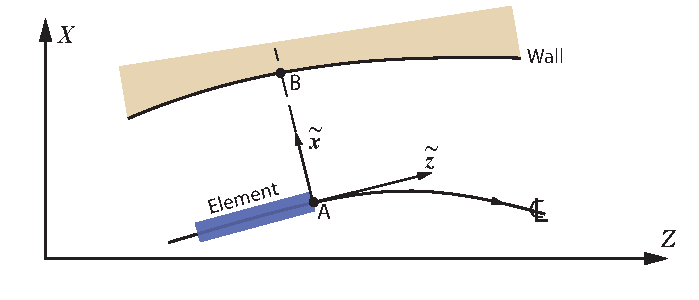
\includegraphics[width=5in]{building-wall-constraint.pdf}
  \caption[Building wall datum]
{A \vn{wall.} datum is a measure of the distance between the
centerline of a machine and the walls of the containment building.}
  \label{f:wall.constraint}
\end{figure}

  %----------------------
  \item[velocity, velocity.x, .y, .z] \Newline \hlabel{velocity}
The velocity normalized by the speed of light $c$.

  %----------------------
  \item[wall.left_side, .right_side] \Newline \hlabel{wall}
The \vn{wall} data data type is used to constrain the shape of a machine to fit inside a building's
walls (\sref{s:building.wall}). The general layout is shown in Figure~\ref{f:wall.constraint}. The
machine centerline is projected onto the horizontal $(Z, X)$ plane in the Global (floor) coordinate
system. Point \vn{A} is an evaluation point at the exit end of some element. $\wt z$ is the
projection of the local $z$-axis onto the $(Z, X)$ plane and $\wt x$ is the coordinate in the $(Z,
X)$ plane perpendicular to $\wt z$. In the typical situation, where a machine is planer (no
out-of-plane bends), the $\wt z$-axis corresponds to the local laboratory $z$-axis and the $\wt
x$-axis corresponds to the local laboratory $x$-axis (see the \bmad manual for an explanation of
local and global coordinate systems).

The distance from the machine at point \vn{A} to the wall is defined to be the distance from \vn{A}
to a point \vn{B} on the wall where point \vn{B} is along the $\wt x$ axis (has $\wt z = 0$) as
shown in Figure~\ref{f:wall.constraint}.

By definition, the \vn{``left side''} of the machine corresponds to be the $+\wt x$ side and the
\vn{``right side''} corresponds to be the $-\wt x$ side. That is, left and right are relative to
someone looking in the same direction as the beam is propagating. Correspondingly, there are two
wall data types: \vn{wall.left_side} and \vn{wall.right_side}. With the \vn{wall.left_side} data
type, the datum value is positive if point \vn{B} is on the left side and negative if on the
right. Vice versa for a \vn{wall.right_side} datum.  That is, there is interference with with wall
when the datum value is negative. If there are multiple wall points \vn{B}, that is, if there are
multiple points on the wall with $\wt z = 0$, the datum value will be the minimum value. Notice that
only wall sections that have a \vn{constraint} matching the datum will be used when searching for
possible points \vn{B}. If there are no wall points with $\wt z = 0$, the datum will be marked
invalid.

For \vn{wall} data there can be no reference element since this does not make sense.

Note: To constrain the machine vertically, use the \vn{floor.y} datum type. To constrain the length of
the machine, use the \vn{s_position} datum type.

  %----------------------
  \item[wire.<angle>] \Newline \hlabel{wire}
\vn{wire} data simulates the measurement of a wire scanner. The angle
specified is the angle of the wire with respect to the horizontal
axis. The measurement then measures the second moment $<uu>$ along an
axis which is 90 degrees off of the wire axis. For example,
\vn{wire.90} is a wire scanner oriented in the vertical direction and
measures the second moment of the beam along the horizontal axis,
$<xx>$. The resultant data is not the beam size, but the beam size
squared.

  \end{description}

%------------------------------------------------------------------------
\section{Data Types Table}
\label{s:data.table}

See the previous section for a description of the data types.

\index{data!calculation method}
\index{unstable.orbit}\index{beta}\index{alpha}\index{eta}\index{eta}
\index{etap}\index{phase}\index{orbit}\index{wire}\index{building wall}\index{spin}
\index{cbar}\index{coupling}\index{floor}\index{r}\index{t}\index{tt}
\index{rad_int.i5a_e6}\index{rad_int.i5b_e6}\index{s_position}\index{e_tot}
\index{emittance}\index{chrom}\index{norm_emittance}
\index{sigma}\index{dpx_dx}\index{dpy_dy}\index{dpz_dz}\index{dpa_da}
\index{dpb_db}\index{rad_int.i1}\index{rad_int.i2}\index{rad_int.i2_e4}
\index{rad_int.i3}\index{rad_int.i3_e7}

%----------------------------------------------------------------------------------------------

{\tt\small
\begin{longtable}{lllll} 
  \caption{Predefined Data Types in Tao}
  \label{t:data.types}
  \\ \hline

  {\it Pg}{\texttt \#}    & {\it Data_Type}                      & {\it Description}   & {\it data_source} & 
                                            \begin{sideways} \parbox{0.6in}{\begin{tabular}{@{}l}
                                            {\it Can use} \\ {\it s_offset?} \end{tabular}} \end{sideways} \\ \hline\hline
  \endfirsthead

  \caption[]{(continued)} \\ \hline
  {\it Pg}{\texttt \#}    & {\it Data_Type}                      & {\it Description}   & {\it data_source} & 
                                            \begin{sideways} \parbox{0.6in}{\begin{tabular}{@{}l}
                                            {\it Can use} \\ {\it s_offset?} \end{tabular}} \end{sideways} \\ \hline\hline
  \endhead

  \pref{alpha}            & alpha.a, .b                         & Normal-Mode alpha function                & lat         & Yes \\ \hline 
  \pref{apparent.emit}    & apparent_emit.x, .y                 & Apparent emittance                        & lat, beam   & No  \\ \hline
  \pref{beta.a}           & beta.a, .b, .c                      & Normal-mode beta function                 & lat, beam   & Yes \\ \hline 
  \pref{beta.x}           & beta.x, .y, .z                      & Projected beta function                   & lat, beam   & No  \\ \hline 
  \pref{bpm.cbar}         & \begin{tabular}{@{}l}   
                              bpm_cbar.22a, .12a, \\
                              \hspace{4em} .11b, .12b
                            \end{tabular}                       & Measured coupling                         & lat         & Yes \\ \hline
  \pref{bpm.eta}          & bpm_eta.x, .y                       & Measured dispersion                       & lat         & Yes \\ \hline
  \pref{bpm.orbit}        & bpm_orbit.x, .y                     & Measured orbit                            & lat         & Yes \\ \hline
  \pref{bpm.phase}        & bpm_phase.a, .b                     & Measured betatron phase                   & lat         & Yes \\ \hline
  \pref{bpm.k}            & \begin{tabular}{@{}l}   
                              bpm_k.22a, .12a, \\
                              \hspace{4em} .11b, .12b   
                             \end{tabular}                      & Measured coupling                         & lat         & Yes \\ \hline
  \pref{bunch.charge}     & \begin{tabular}{@{}l}   
                              bunch_charge.live, \\
                              \hspace{4em} .live_relative
                            \end{tabular}                       & Charge of live particles                  & beam        & No  \\ \hline
  \pref{bunch.max}        & \begin{tabular}{@{}l}   
                              bunch_max.x, .y, .z, \\ 
                              \hspace{4em} .px, .py, .pz  
                            \end{tabular}                       & Max relative to centroid                  & beam        & No  \\ \hline
  \pref{bunch.min}        & \begin{tabular}{@{}l}
                              bunch_min.x, .y, .z, \\ 
                              \hspace{4em} .px, .py, .pz
                            \end{tabular}                       & Min relative to centroid                  & beam        & No  \\ \hline
  \pref{cmat}             & cmat.11, .12, .21, .22              & Coupling matrix elements                  & lat         & Yes \\ \hline 
  \pref{cmat}             & cbar.11, .12, .21, .22              & Normalized coupling matrix                & lat         & Yes \\ \hline 
  \pref{chrom.a}          & chrom.a, .b                         & Chromaticities for a ring                 & lat         & No  \\ \hline
  \pref{chrom.dbeta}      & chrom.dbeta.a, .dbeta.b             & Normalized Chromatic beta                 & lat         & No  \\ \hline
  \pref{chrom.deta}       & chrom.deta.x, .deta.y               & Chromatic dispersions                     & lat         & No  \\ \hline
  \pref{chrom.detap}      & chrom.detap.x, .detap.y             & Chromatic dispersion slopes               & lat         & No  \\ \hline
  \pref{chrom.dphi}       & chrom.dphi.a, .dphi.b               & Chromatic betatron phase                  & lat         & No  \\ \hline
  \pref{chrom.w}          & chrom.w.a, .w.b                     & Chromatic W-functions                     & lat         & No  \\ \hline
  \pref{chrom.ptc}        & \begin{tabular}{@{}l}
                              chrom_ptc.a.$N$, \\
                              chrom_ptc.b.$N$, \\
                              \hspace{4em} $N = 0, 1, \ldots$
                            \end{tabular}                       & Chromaticity Taylor terms                 & lat         & no  \\ \hline
  \pref{curly.h}          & curly_h.a, .b                       & \begin{tabular}{@{}l}
                                                                    Radiation integrals \\
                                                                    curly H function 
                                                                  \end{tabular}                             & lat         & Yes \\ \hline
  \pref{damp}             & damp.j_a, .j_b, .j_z                & Damping partition number                  & lat         & No  \\ \hline
  \pref{dpx.dx}           & dpx_dx, dpx_dy, etc.                & Bunch <x px> / <$x^2$> \& Etc...          & beam        & No  \\ \hline 
  \pref{da}               & \begin{tabular}{@{}l}
                              dynamic_aperture.$N$, \\
                              \hspace{4em} $N = 1, 2, 3 \ldots$
                            \end{tabular}                       & Dynamic aperture                          & lat         & No  \\ \hline
  \pref{e.tot.ref}        & e_tot_ref                           & Lattice reference energy (eV)             & lat         & No  \\ \hline
  \pref{element.attrib}   & element_attrib.<attr_name>          & lattice element attribute                 & lat         & No  \\ \hline
  \pref{emit.a}           & emit.a, .b, .c                      & Emittance                                 & lat, beam   & No  \\ \hline
  \pref{emit.x}           & emit.x, .y, .z                      & Projected emittance                       & lat, beam   & No  \\ \hline
  \pref{eta.x}            & eta.x, .y, .z                       & Dispersion                                & lat, beam   & Yes \\ \hline 
  \pref{eta.a}            & eta.a, .b                           & Normal-mode dispersion                    & lat, beam   & Yes \\ \hline 
  \pref{etap.x}           & etap.x, .y                          & Dispersion derivative                     & lat, beam   & Yes \\ \hline 
  \pref{etap.a}           & etap.a, .b                          & \begin{tabular}{@{}l}   
                                                                    dispersion derivative
                                                                  \end{tabular}                             & lat, beam   & Yes \\ \hline 
  \pref{expression}       & expression:<expression>             & See text above                            & lat         & No  \\ \hline 
  \pref{floor}            & \begin{tabular}{@{}l}   
                              floor.x, .y, .z, \\             
                              \hspace{2em} theta, .phi, .psi
                            \end{tabular}                       & \begin{tabular}{@{}l}   
                                                                    Lattice element \\
                                                                    global position
                                                                   \end{tabular}                            & lat         & Yes \\ \hline
  \pref{floor.actual}     & \begin{tabular}{@{}l}
                              floor_actual.x, .y, .z, \\
                              \hspace{3em} .theta, .phi, .psi 
                            \end{tabular}                       & \begin{tabular}{@{}l}   
                                                                    Lattice element \\ 
                                                                    misaligned global position
                                                                  \end{tabular}                             & lat         & Yes \\ \hline 
  \pref{floor.orbit.x}    & floor_orbit.x, .y, .z               & global position of orbit                  & lat, beam   & Yes \\ \hline 
  \pref{floor.orbit.t}    & \begin{tabular}{@{}l}   
                              floor_orbit.theta, \\
                              \hspace{3em} .phi, .psi 
                            \end{tabular}                       & global position of orbit                  & lat, beam   & Yes \\ \hline 
  \pref{gamma}            & gamma.a, .b                         & Normal-mode gamma function                & lat         & Yes \\ \hline 
  \pref{k.11b}            & k.11b, .12a, .12b, .22a             & Coupling                                  & lat         & Yes \\ \hline   
  \pref{momentum}         & momentum                            & Momentum: P*C_light (eV)                  & lat         & Yes \\ \hline
  \pref{mom.comp}         & momentum_compaction                 & Momentum compaction factor                & lat         & No  \\ \hline
  \pref{mom.comp.ptc}     & \begin{tabular}{@{}l}
                              momentum_compaction_ptc.$N$ \\
                              \hspace{3em} $N = 0, 1, 2, \ldots$
                            \end{tabular}                       & \begin{tabular}{@{}l}
                                                                    Momentum compaction \\
                                                                    Taylor terms
                                                                  \end{tabular}                             & lat         & No  \\ \hline
  \pref{multi.turn.orb}   &  \begin{tabular}{@{}l}
                               multi_turn_orbit.x, .y, \\ 
                               \hspace{3em} .z, .px, .py, .pz
                             \end{tabular}                      & Store orbit over many turns               & lat         & No  \\ \hline 
  \pref{n.part.loss}      & n_particle_loss                     & Number of particles lost                  & beam        & No  \\ \hline 
  \pref{norm.app.emit}    & norm_apparent_emit.x, .y            & Normalized apparent emittance             & lat, beam   & No  \\ \hline
  \pref{norm.emit.a}      & norm_emit.a, .b, .c                 & Normalized beam emittance                 & lat, beam   & No  \\ \hline 
  \pref{norm.emit.x}      & norm_emit.x, .y, .z                 & Normalized projected emittance            & lat, beam   & No  \\ \hline 
  \pref{normal.type}      & normal.<type>.$i$.<monomial>        & Normal form map component                 & lat         & No  \\ \hline
  \pref{normal.h}         & normal.h.<monomial>                 & Normal form driving term                  & lat         & No  \\ \hline
  \pref{null}             & null                                & Data without model evaluation             & lat, beam   & No  \\ \hline
  \pref{orbit.e.tot}      & orbit.e_tot                         & Beam energy (eV)                          & lat, beam   & Yes \\ \hline
  \pref{orbit.x}          & \begin{tabular}{@{}l}
                              orbit.x, .y, .z \\
                              \hspace{3em} .px, .py, .pz
                            \end{tabular}                       & Phase space orbit                         & lat, beam   & Yes \\ \hline 
  \pref{orbit.amp}        & orbit.amp_a, .amp_b                 & Orbit amplitude                           & lat         & Yes \\ \hline 
  \pref{orbit.norm.amp}   & \begin{tabular}{@{}l}
                              orbit.norm_amp_a, \\
                              \hspace{2em} .norm_amp_b       
                            \end{tabular}                       & Energy normalized amplitude               & lat         & Yes \\ \hline 
  \pref{periodic.tt}      & \begin{tabular}{@{}l}
                              periodic.tt.$ijklm\ldots$ \\
                              \hspace{4em} $1 \le i,j,k,\ldots \le 6$   
                            \end{tabular}                       & Periodic map Taylor terms                 & lat         & No  \\ \hline 
  \pref{phase}            & phase.a, .b                         & Betatron phase                            & lat         & Yes \\ \hline 
  \pref{phase.frac}       & phase_frac.a, .b                    & \begin{tabular}{@{}l}
                                                                    Fractional betatron phase \\       
                                                                    $-\pi < \phi_{\mbox{frac}} < \pi$ 
                                                                  \end{tabular}                             & lat         & No  \\ \hline 
  \pref{phase.frac.diff}  & phase_frac_diff                     & \begin{tabular}{@{}l}
                                                                    Phase difference \\
                                                                    between $a$ and $b$ modes
                                                                  \end{tabular}                             & lat         & No  \\ \hline 
  \pref{photon.intens}    & photon.intensity                    & Photon total intensity                    & lat, beam   & No  \\ \hline 
  \pref{photon.intens.x}  & \begin{tabular}{@{}l}
                              photon.intensity_x, \\
                              \hspace{2em} .intensity_y
                            \end{tabular}                       & Photon intensity components               & lat, beam   & No  \\ \hline
  \pref{photon.phase}     & photon.phase_x, .phase_y            & Photon phase                              & lat, beam   & No  \\ \hline  
  \pref{ping.a}           & \begin{tabular}{@{}l}
                              ping_a.amp_x, .phase_x,                  \\
                              \hspace{1.5em} .amp_y, .phase_y,         \\
                              \hspace{1.5em} .amp_sin_y, .amp_cos_y,   \\
                              \hspace{1.5em} .amp_sin_rel_y,           \\
                              \hspace{1.5em} .amp_cos_rel_y 
                            \end{tabular}                       & Pinged beam $a$-mode response             & lat        & No  \\ \hline
  \pref{ping.b}           & \begin{tabular}{@{}l}
                              ping_b.amp_x, .phase_x,                 \\
                              \hspace{1.5em} .amp_y, .phase_y,        \\
                              \hspace{1.5em} .amp_sin_x, .amp_cos_x,  \\
                              \hspace{1.5em} .amp_sin_rel_x,          \\
                              \hspace{1.5em} .amp_cos_rel_x 
                            \end{tabular}                       & Pinged beam $b$-mode response             & lat        & No  \\ \hline
  \pref{r.ij}             & r.$ij$ \hspace{10pt} $1 \le i,j \le 6$ & Term in linear transfer map            & lat        & Yes \\ \hline 
  \pref{r56.comp}         & r56_compaction                        & R56 like compaction factor.             & lat        & No  \\ \hline
  \pref{rad.int}          & rad_int.i1, .i2, etc.               & Lattice Radiation integrals               & lat        & No  \\ \hline
  \pref{rad.int1}         & rad_int1.i1, .i2, etc.              & Element radiation integrals               & lat        & No  \\ \hline
  \pref{ref.time}         & ref_time                            & Reference time                            & lat, beam  & Yes \\ \hline
  \pref{rel.floor}        & \begin{tabular}{@{}l}
                              rel_floor.x, .y, \\
                              \hspace{4em} .z, .theta
                            \end{tabular}                       & Relative global floor position            & lat        & No  \\ \hline 
  \pref{s.position}       & s_position                          & longitudinal length constraint            & lat        & Yes \\ \hline 
  \pref{sigma}            & \begin{tabular}{@{}l}   
                              sigma.x, .y, .z, \\
                              \hspace{2em} .px, px, .pz, \\
                              \hspace{2em} .$ij$ \hspace{10pt} $1 \le i,j \le 6$, \\
                              \hspace{2em} .Lxy
                            \end{tabular}                       & Bunch size                                & lat, beam  & No  \\ \hline 
  \pref{spin}             & spin.x, .y, .z                      & Particle spin                             & lat, beam  & No  \\ \hline 
  \pref{spin.pol}         & spin.depolarization_rate            & Spin depolarization rate.                 & lat        & No  \\ \hline
  \pref{spin.pol}         & spin.polarization_rate              & Spin polarization rate.                   & lat        & No  \\ \hline
  \pref{spin.pol}         & spin.polarization_limit             & Spin polarization limit.                  & lat        & No  \\ \hline
  \pref{spin.tune.ptc}    & \begin{tabular}{@{}l}
                              spin_tune_ptc.$N$, \\
                              \hspace{10pt} $N = 0, 1, \ldots$
                            \end{tabular}                       & Spin Tune Taylor terms                    & lat        & no  \\ \hline
  \pref{spin.g.matrix}    & \begin{tabular}{@{}l}   
                              spin_g_matrix.$ij$ \\
                              \hspace{10pt} $1 \le i \le 2$, $1 \le j \le 6$ 
                            \end{tabular}                       & Spin G-matrix components                  & lat        & No  \\ \hline
  \pref{srdt.h}           & srdt.h<monomial>.\{r,i,a\}          & \begin{tabular}{@{}l}
                                                                    Normal form driving terms \\
                                                                    calculated by summation 
                                                                  \end{tabular}                             & lat        & No \\ \hline
  \pref{time}             & time                                & Particle time (sec)                       & lat, beam  & Yes \\ \hline
  \pref{t.ijk}            & \begin{tabular}{@{}l}   
                              t.$ijklm\ldots$, \\
                              tt.$ijklm\ldots$, \\
                            \hspace{4em} $1 \le i,j,k,\ldots \le 6$  
                            \end{tabular}                       & \begin{tabular}{@{}l}
                                                                    Term in n\Th \\
                                                                    order transfer map
                                                                  \end{tabular}                             & lat        & No  \\ \hline 
  \pref{tune}             & tune.a, .b                          & Tune                                      & lat        & No  \\ \hline 
  \pref{unstable.eigen}   & \begin{tabular}{@{}l}
                              unstable.eigen, .eigen.a,  \\
                              \hspace{3em} .eigen.b, .eigen.c
                            \end{tabular}                       & Maximum eigenvalue amplitude              & lat        & No  \\ \hline
  \pref{unstable.lat}     & unstable.lattice                    & \begin{tabular}{@{}l}
                                                                    Positive if \\
                                                                    lattice is unstable
                                                                  \end{tabular}                             & lat        & No  \\ \hline
  \pref{unstable.orbit}   & unstable.orbit                      & \begin{tabular}{@{}l}   
                                                                    Nonzero if particles are \\
                                                                    lost in tracking
                                                                  \end{tabular}                             & lat        & No  \\ \hline
  \pref{velocity}         & velocity                            & Normalized velocity $v/c$                 & lat, beam  & Yes \\ \hline
  \pref{velocity}         & velocity.x, .y, .z                  & Normalized velocity component             & lat, beam  & Yes \\ \hline
  \pref{wall}             & \begin{tabular}{@{}l}   
                              wall.left_side, \\
                              \hspace{4em} .right_side
                            \end{tabular}                       & Building wall constraint                  & lat        & No  \\ \hline
  \pref{wire}             & wire.<angle>                        & Wire scanner at <angle>                   & beam       & No  \\ \hline
\end{longtable}
}
